\documentclass[a4paper,oneside]{article}
\usepackage[left=30mm,right=30mm,top=30mm,bottom=45mm]{geometry}
\usepackage[T1]{fontenc}
\usepackage[utf8]{inputenc}
\usepackage{pdfpages}
\usepackage{tikz}
\usepackage[sfdefault,light]{FiraSans}
\usepackage{FiraMono}
\usepackage{a3pages}
\usepackage{pdflscape}
\usepackage[%
        bookmarksnumbered=true,
        colorlinks=true,
        linkcolor=cyan!50!blue,
        citecolor=violet,
        urlcolor=purple,
    ]{hyperref}

\newcommand\code[1]{\texttt{#1}}

\title{Including PDF Documents In \LaTeX}
\author{Raphael Frey\\[2mm]\small%
    \href{https://github.com/alpenwasser/TeX/tree/master/include-pdfs}
         {\nolinkurl{https://github.com/alpenwasser/TeX}}}

\begin{document}
\maketitle

\tableofcontents

\section{Overview}

Including PDF documents  can be done in  various ways, three of  which will be
presented here and have their advantages and drawbacks discussed.

\begin{itemize}
    \item
        They can be  included as regular images  with the \code{\textbackslash
        includegraphics}   command. This  has   the   advantage  of   allowing
        convenient  scaling  and integration  in  the  text,  and as  such  is
        well-suited for PDF documents which are indeed actual pictures.

        It does, however,  not conveniently allow to include pages  from a PDF
        document as  if they were  pages from the  main document, or  to scale
        them to truly use the full page.
    \item
        One may use  the \code{pdfpages} package. This allows  to insert pages
        from PDF files more or less as if they were part of the main document.
    \item
        Lastly, by  using Ti\emph{k}Z  and overlaying  the included  PDF files
        over the page. Compared  to the \code{pdfpages} package,  this has the
        effect of allowing  annotations and still having  the existing headers
        and footers of  the main document (if the included  PDF does not cover
        them). This may be desirable or not. However, this approach only works
        for single pages.
\end{itemize}

% -------------------------------------------------------------------------- %
\clearpage
\section{Including as Image}
\label{sec:includegraphics}
% -------------------------------------------------------------------------- %

Pretty straightforward, see Figure \ref{fig:includegraphics}.

\begin{figure}[h!]
    \centering
    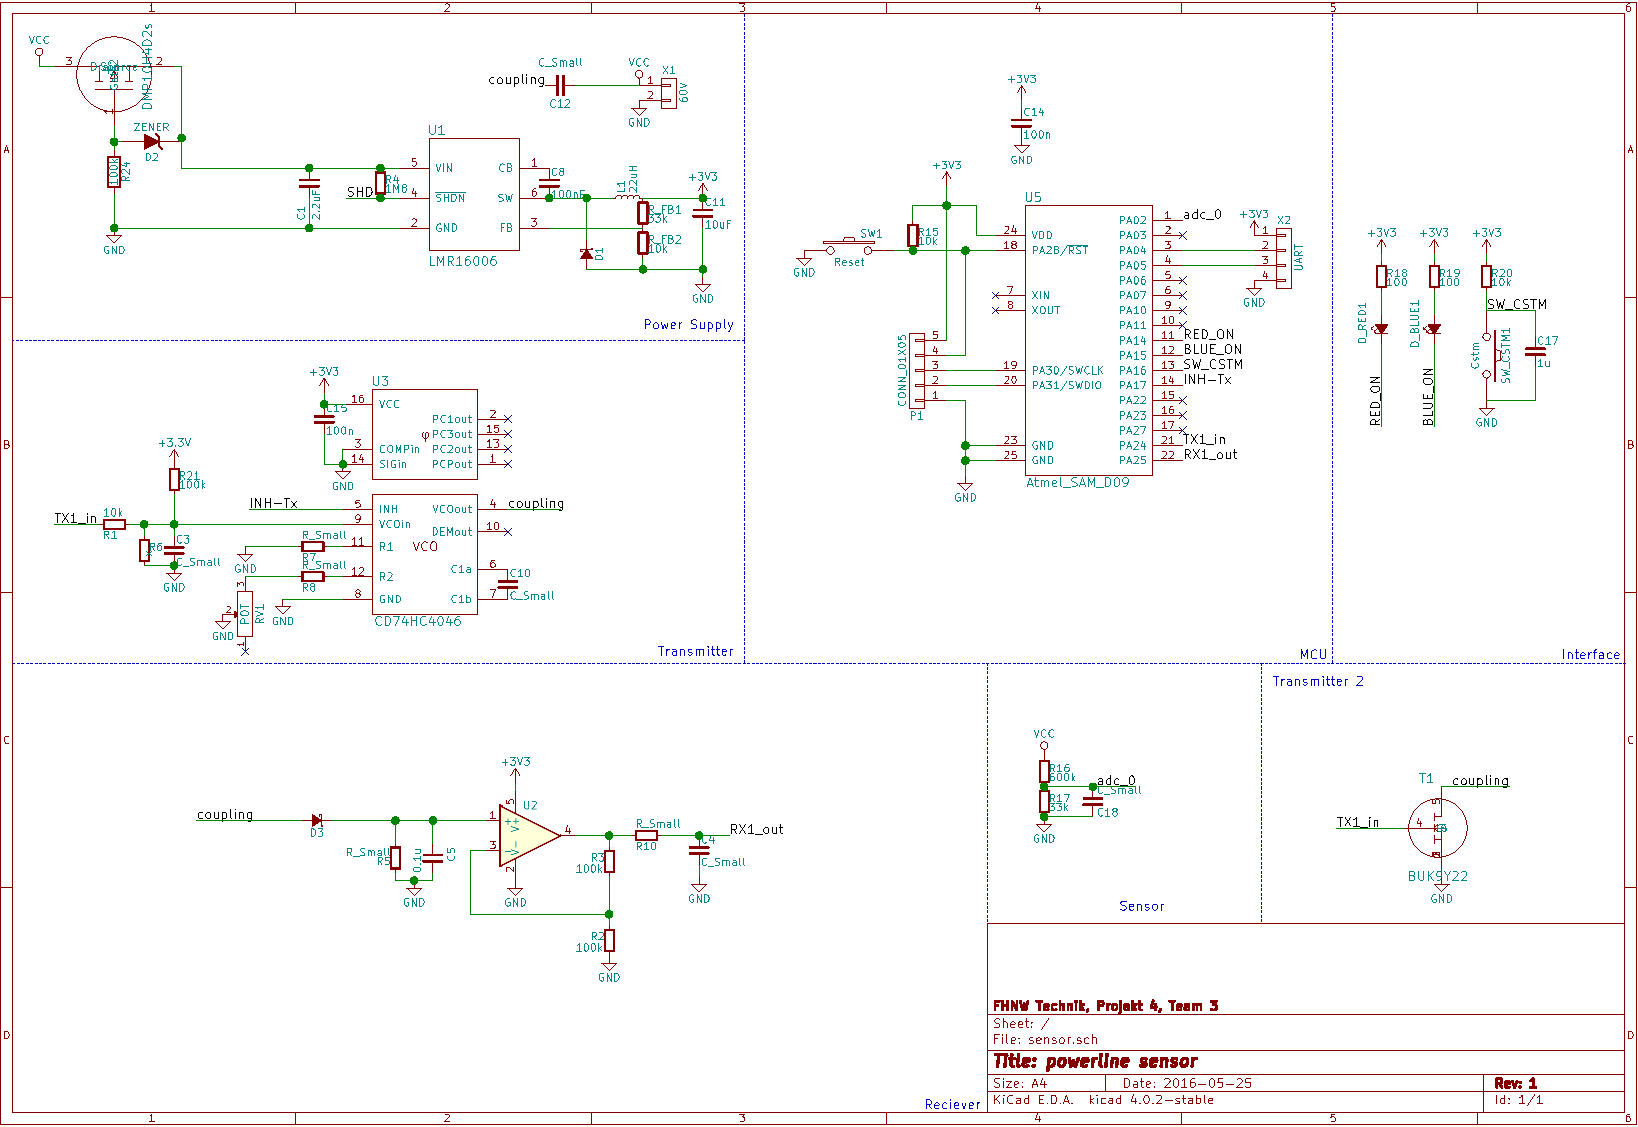
\includegraphics[width=0.75\textwidth]{includes/a4.pdf}
    \caption{%
        This  PDF   file  has   been  included  with   a  \code{\textbackslash
        includegraphics} command.}
    \label{fig:includegraphics}
\end{figure}


% -------------------------------------------------------------------------- %
\clearpage
\section{pdfpages}
\label{sec:pdfpages}
% -------------------------------------------------------------------------- %

For   the    full   range   of    available   package   options,    of   which
there   are    many,   consult   the    manual,   which   is    available   at
\href{http://ctan.org/pkg/pdfpages}{\nolinkurl{http://ctan.org/pkg/pdfpages}}.

The  following command  is used  to  include the  first page  of a  multi-page
document.  The included page is the next page.

\begin{verbatim}
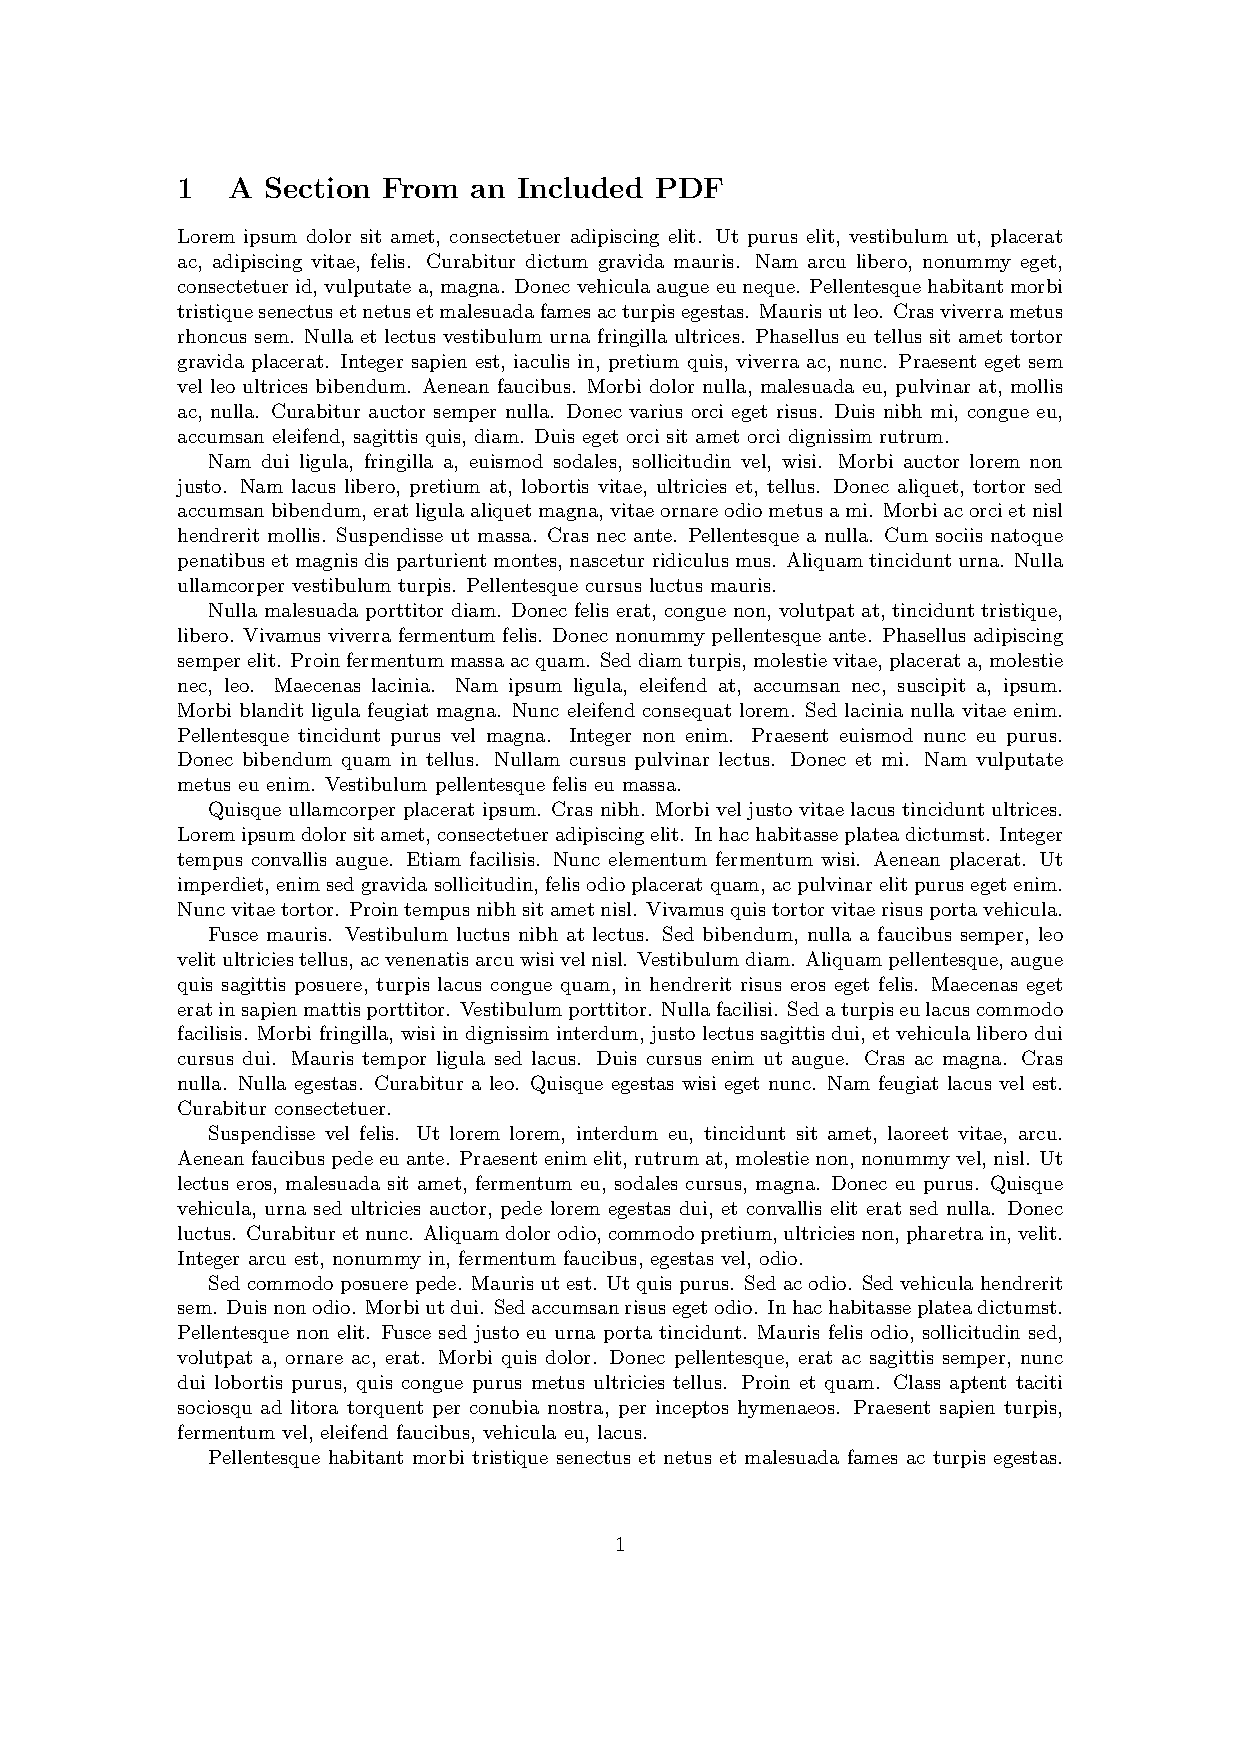
\includepdf[pages={1}]{includes/lipsum.pdf}
\end{verbatim}

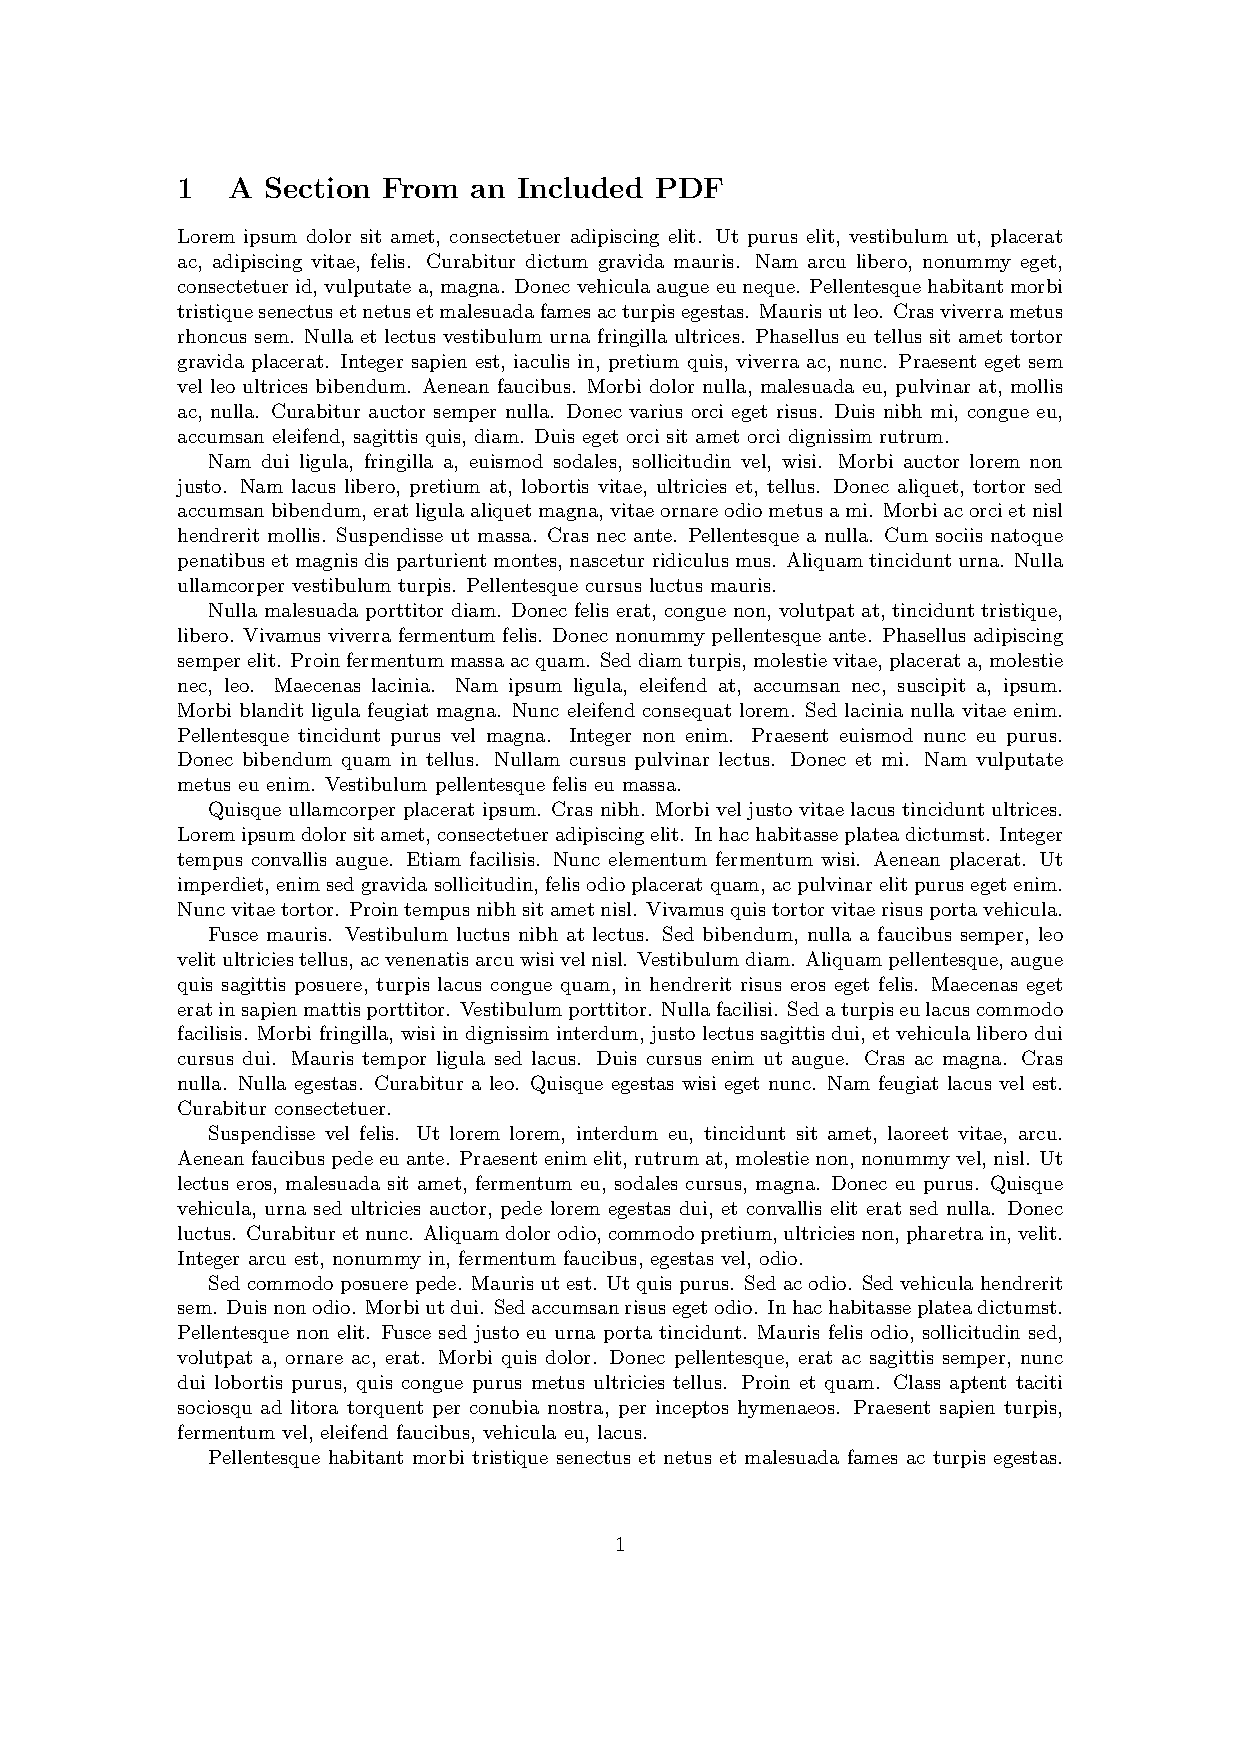
\includepdf[pages={1}]{includes/lipsum.pdf}

The next two pages  include  all pages of an external PDF in  a 2 by 2 grid. A
frame is put around each page. The command used is:

\begin{verbatim}
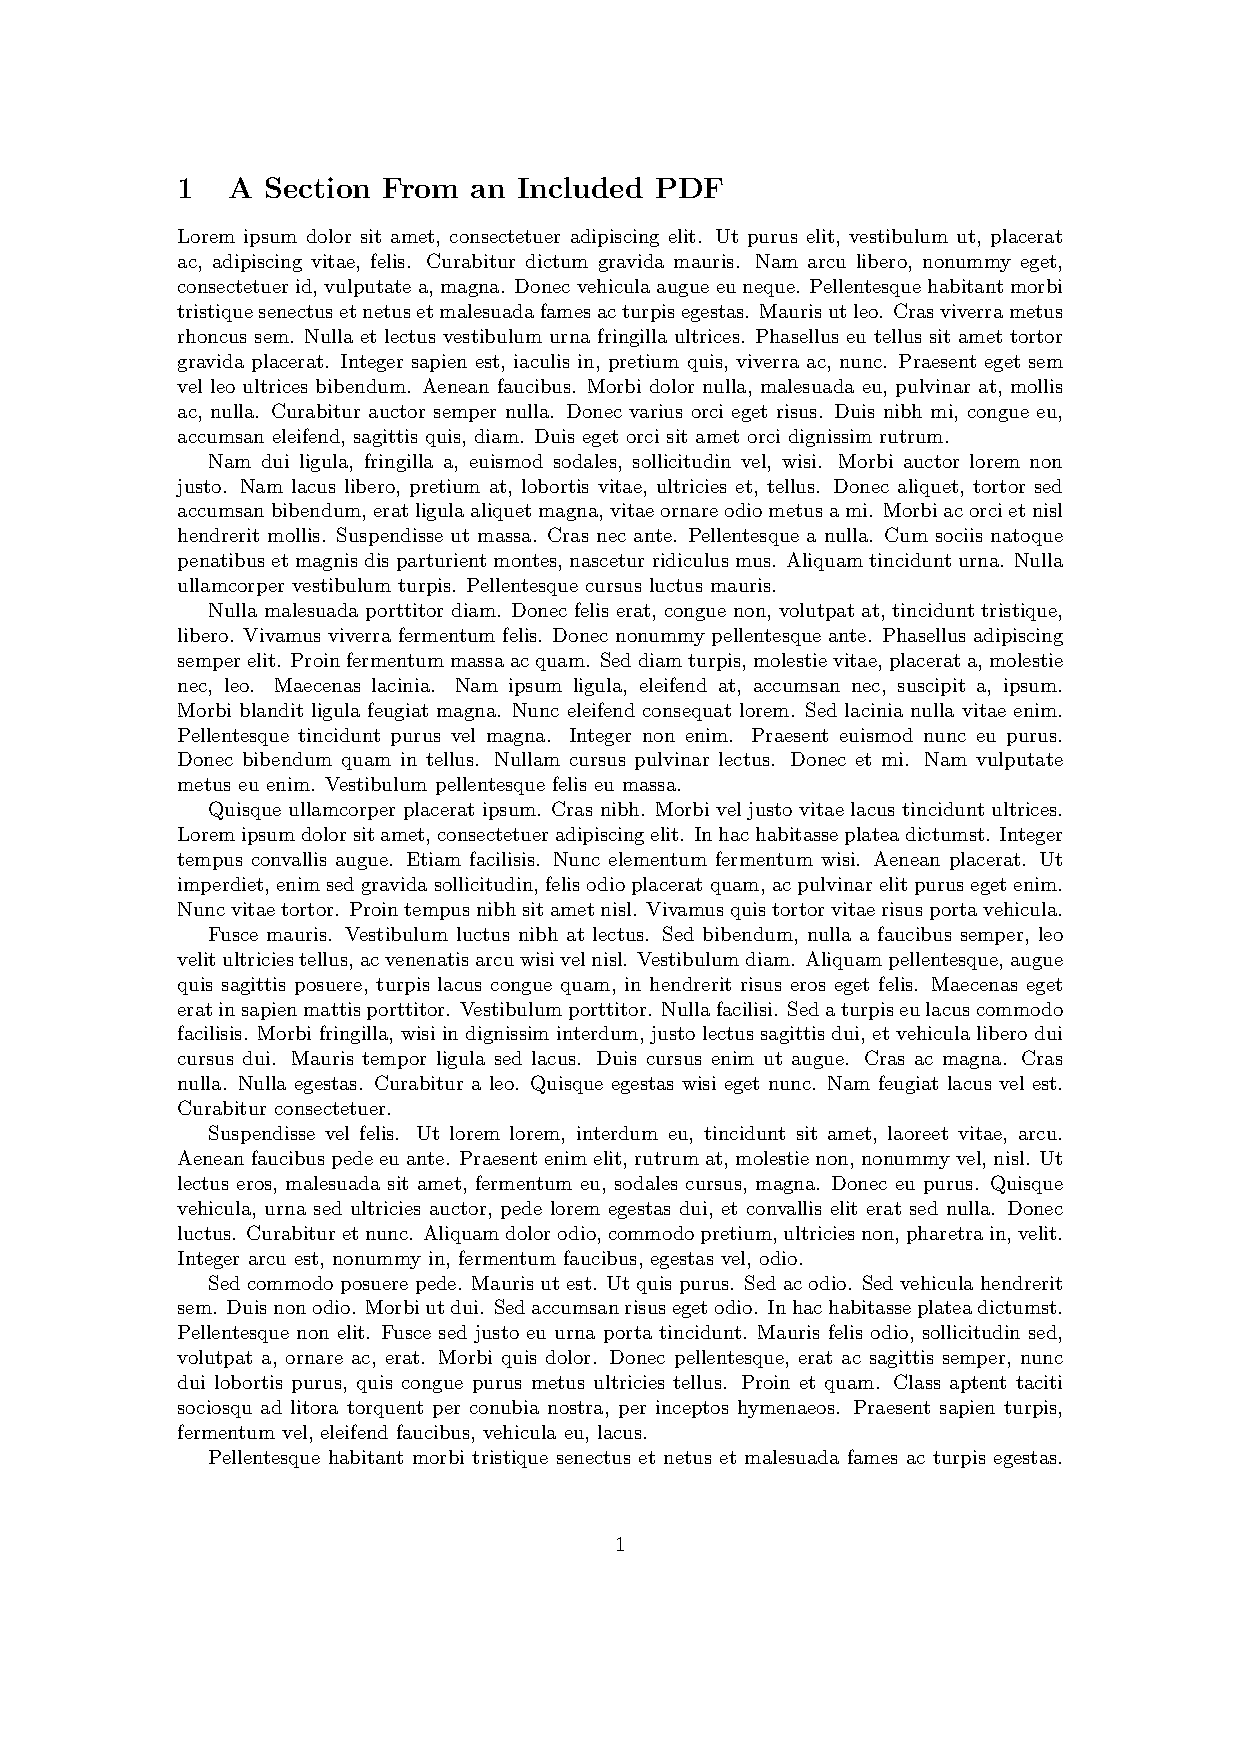
\includepdf[frame,nup=2x2,pages=-}]{includes/lipsum.pdf}
\end{verbatim}

Note that  the page numbering on  the main document includes  the included pdf
pages, even if  their page numbers are  false (due to being  from the included
document, obviously).

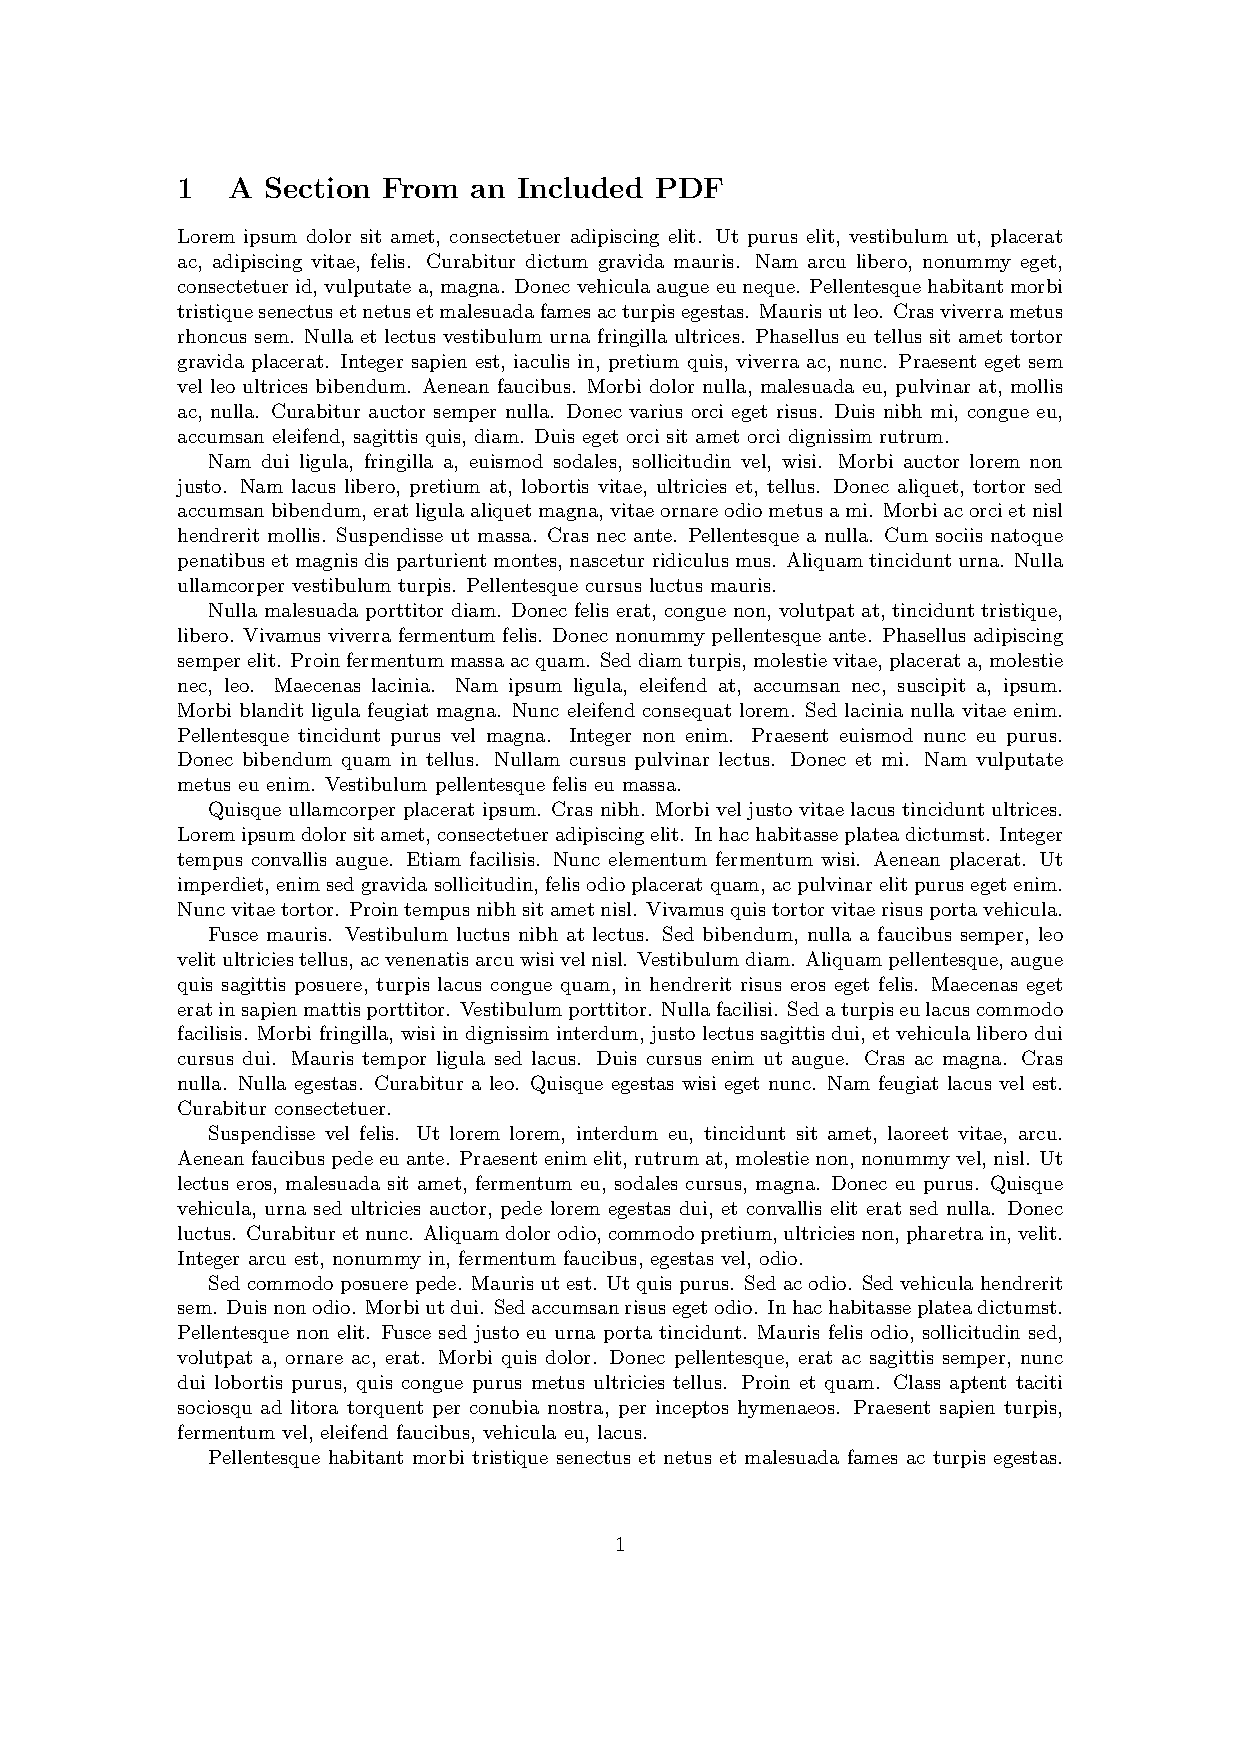
\includepdf[frame,nup=2x2,pages=-]{includes/lipsum.pdf}

Including a landscape document in a portrait  main document can be done in two
ways.  Either tell \code{pdfpages} that the included page is landscape:

\begin{verbatim}
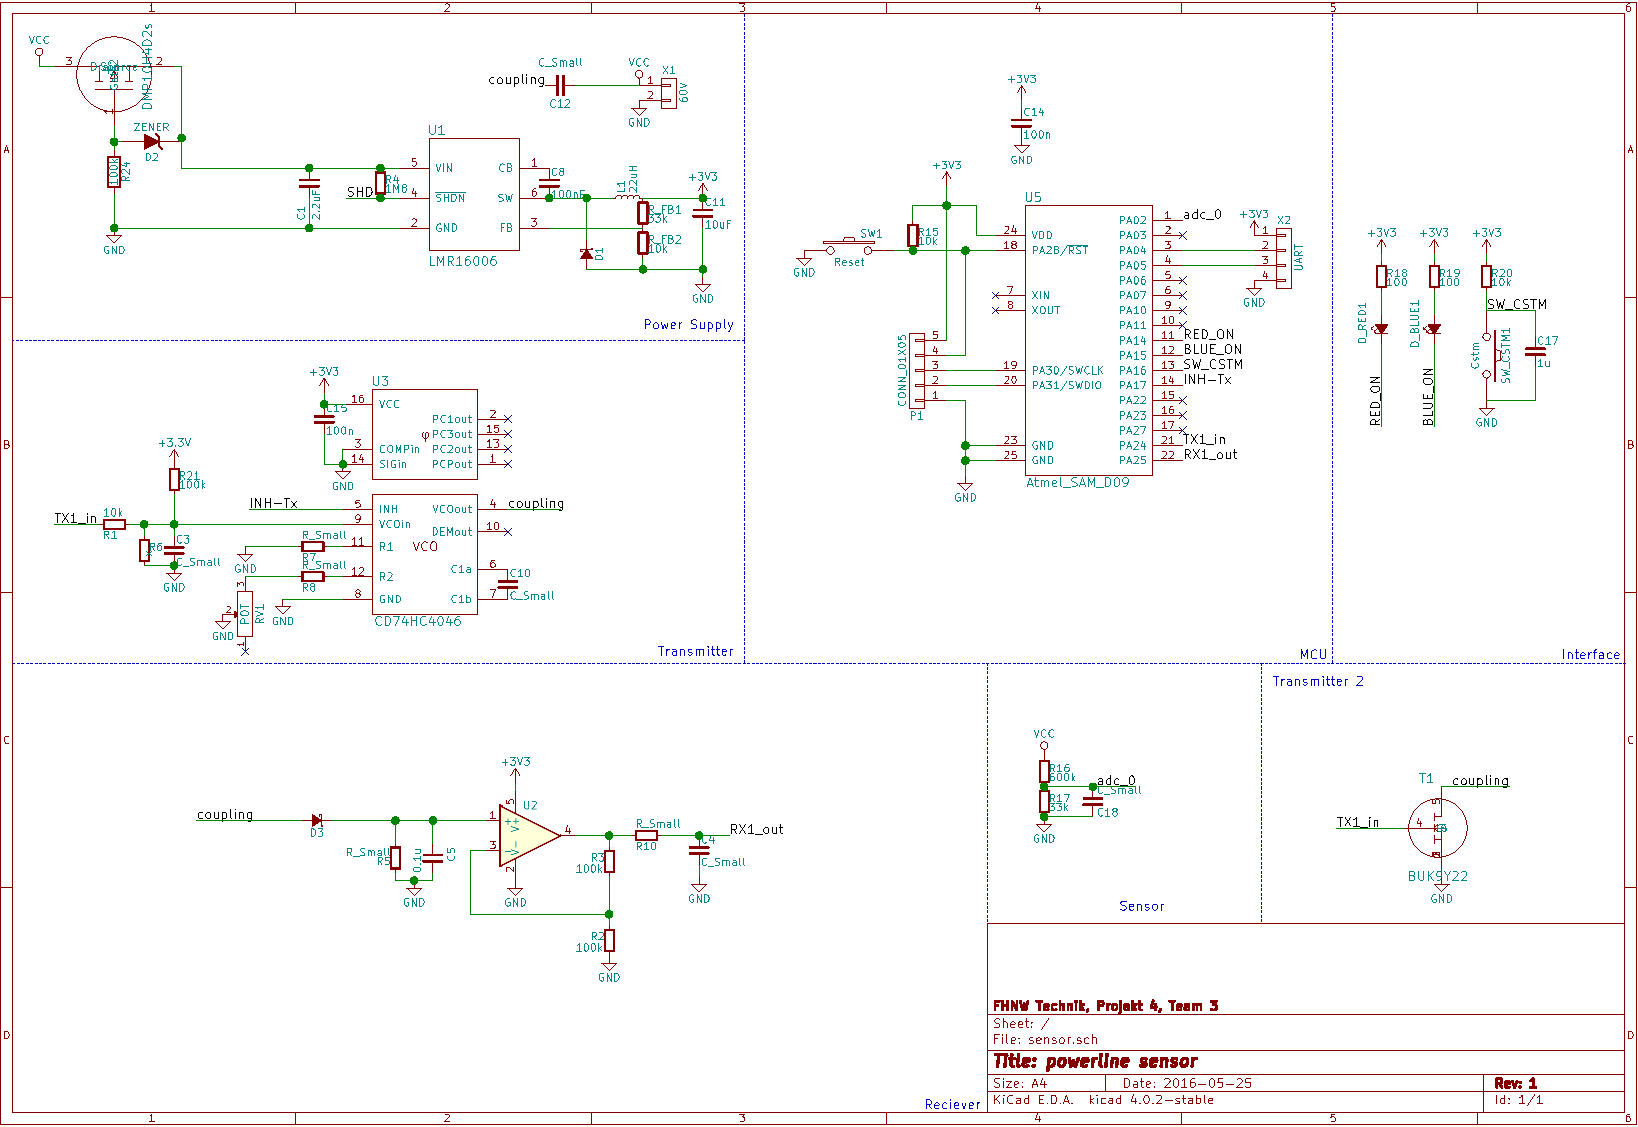
\includepdf[landscape]{includes/a4.pdf}
\end{verbatim}

This will result in the PDF page in the main document being rotated to fit the
included landscape page.

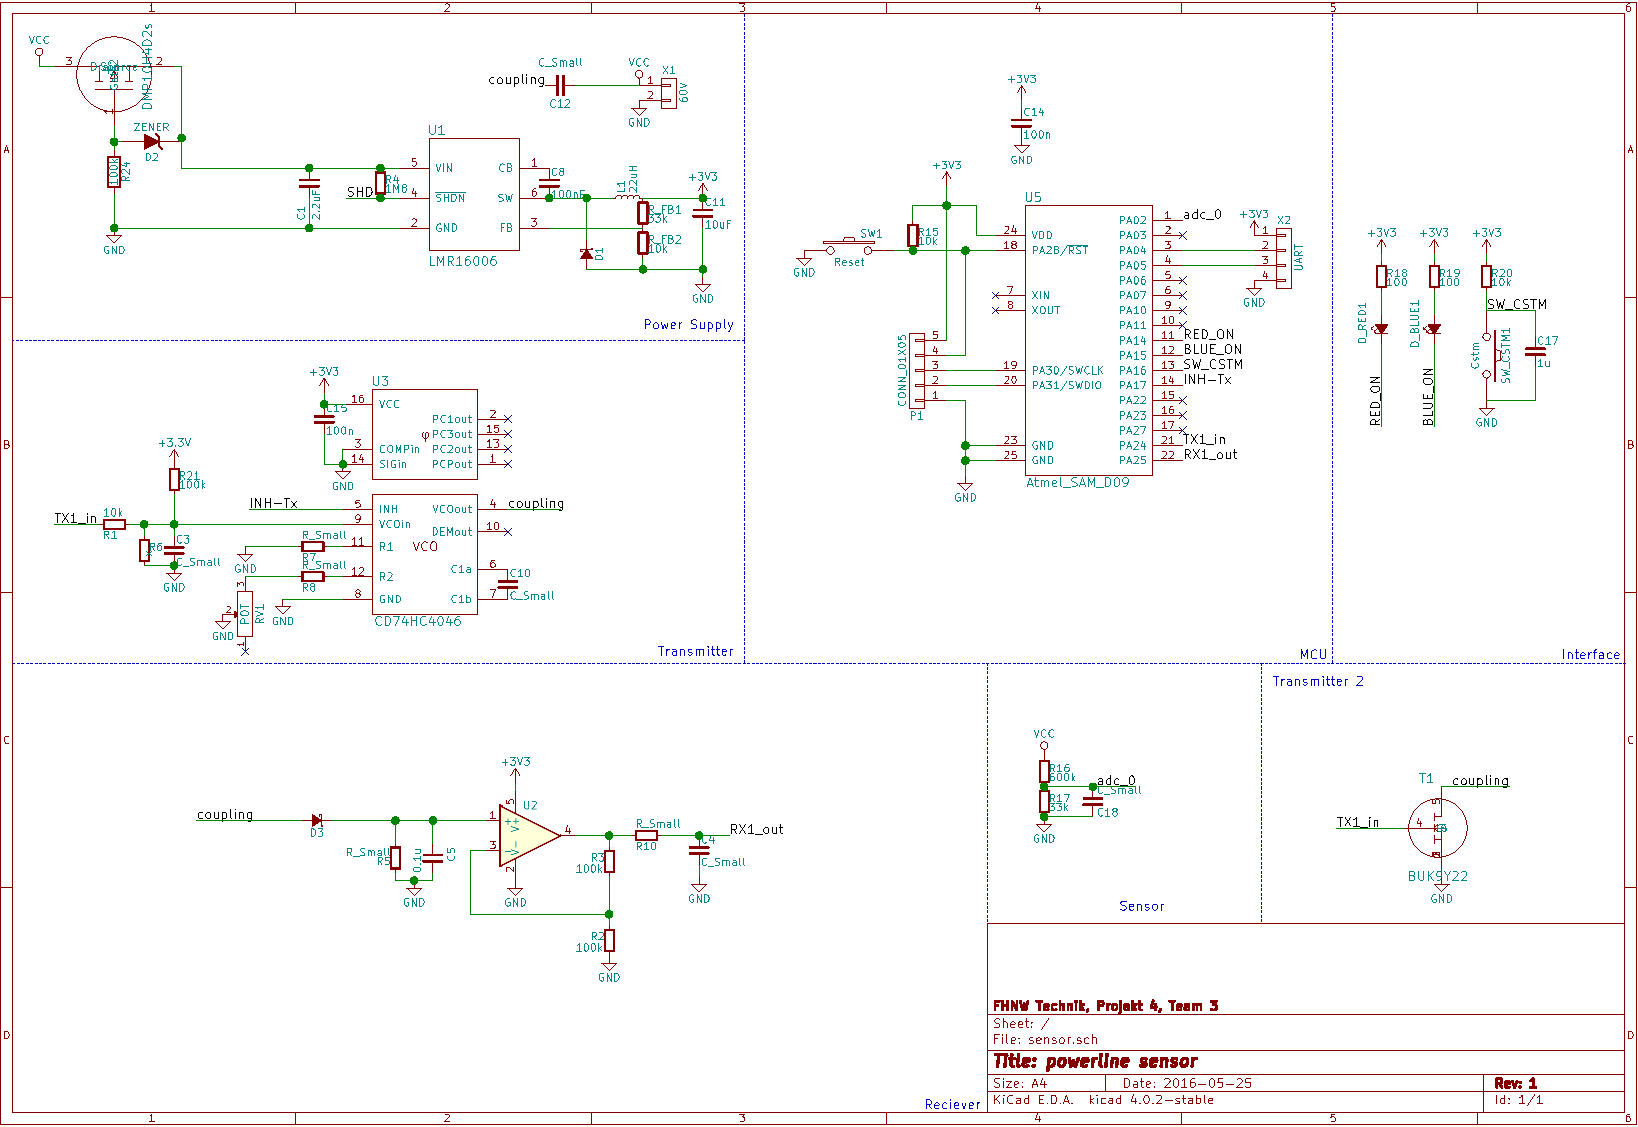
\includepdf[landscape]{includes/a4.pdf}

Alternatively, we can rotate the included  page, which will result in the main
document's page still being in portrait mode:

\begin{verbatim}
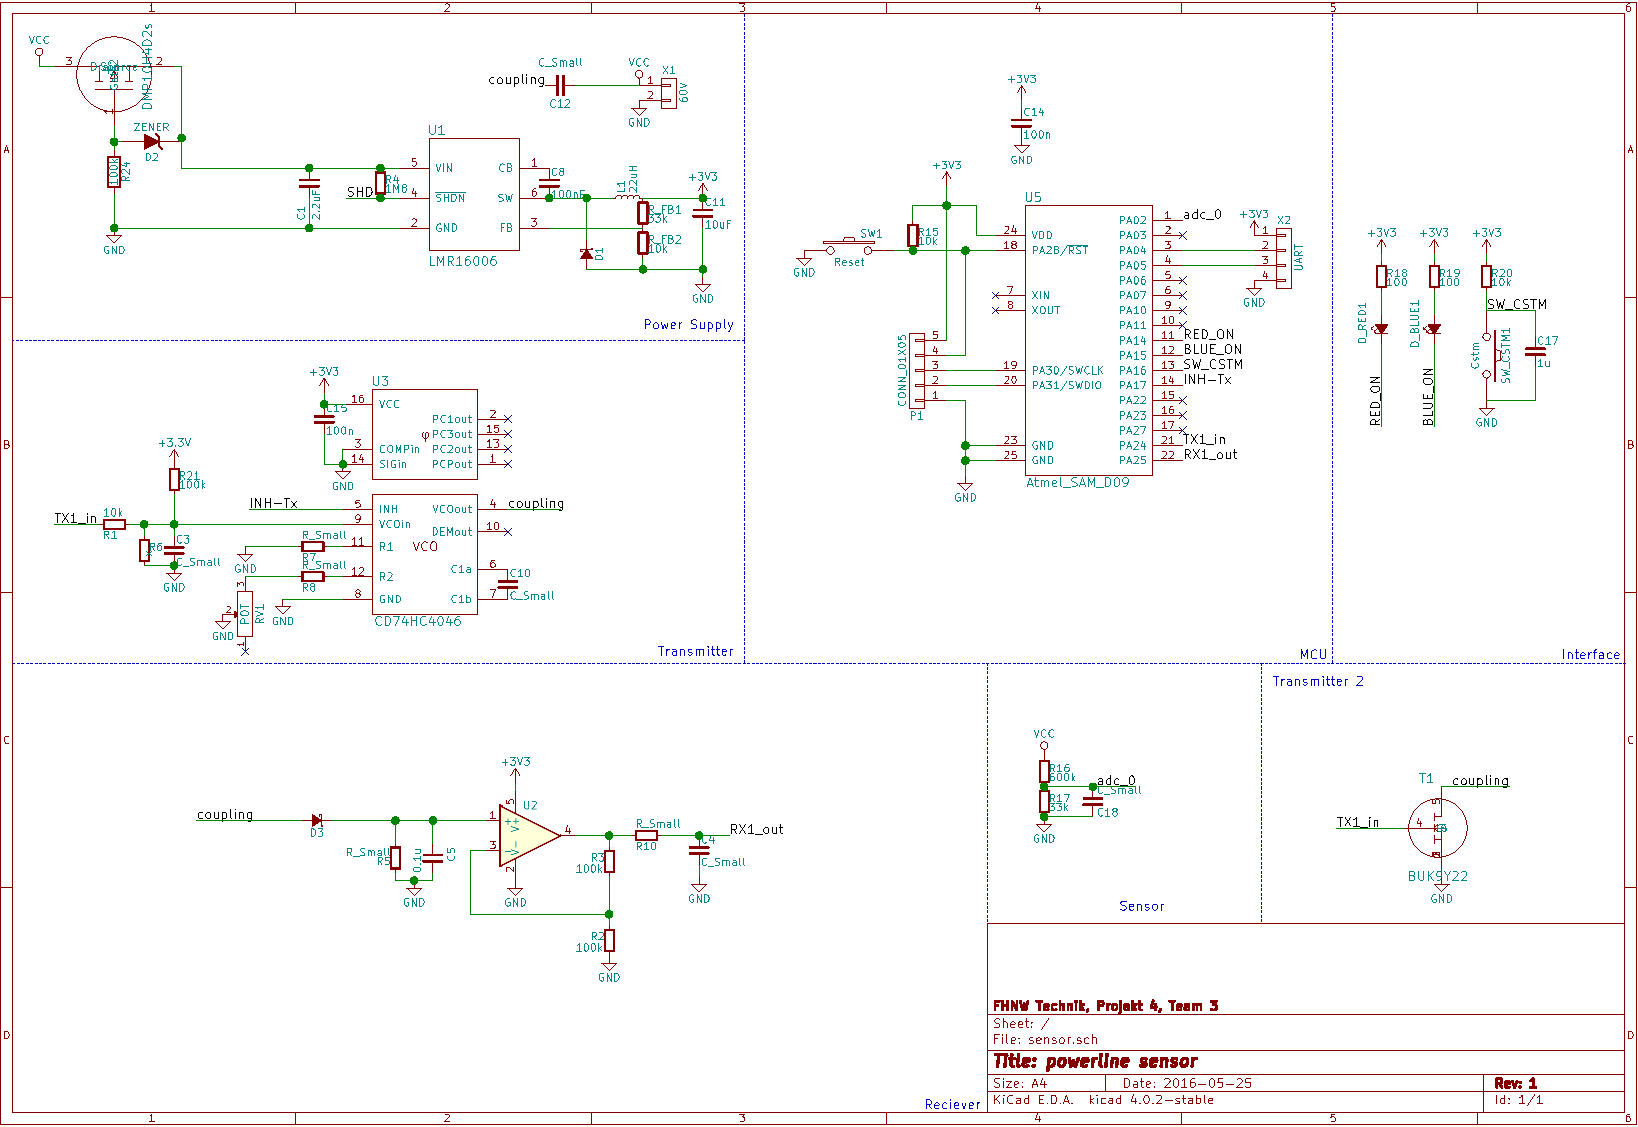
\includepdf[angle=90]{includes/a4.pdf}
\end{verbatim}

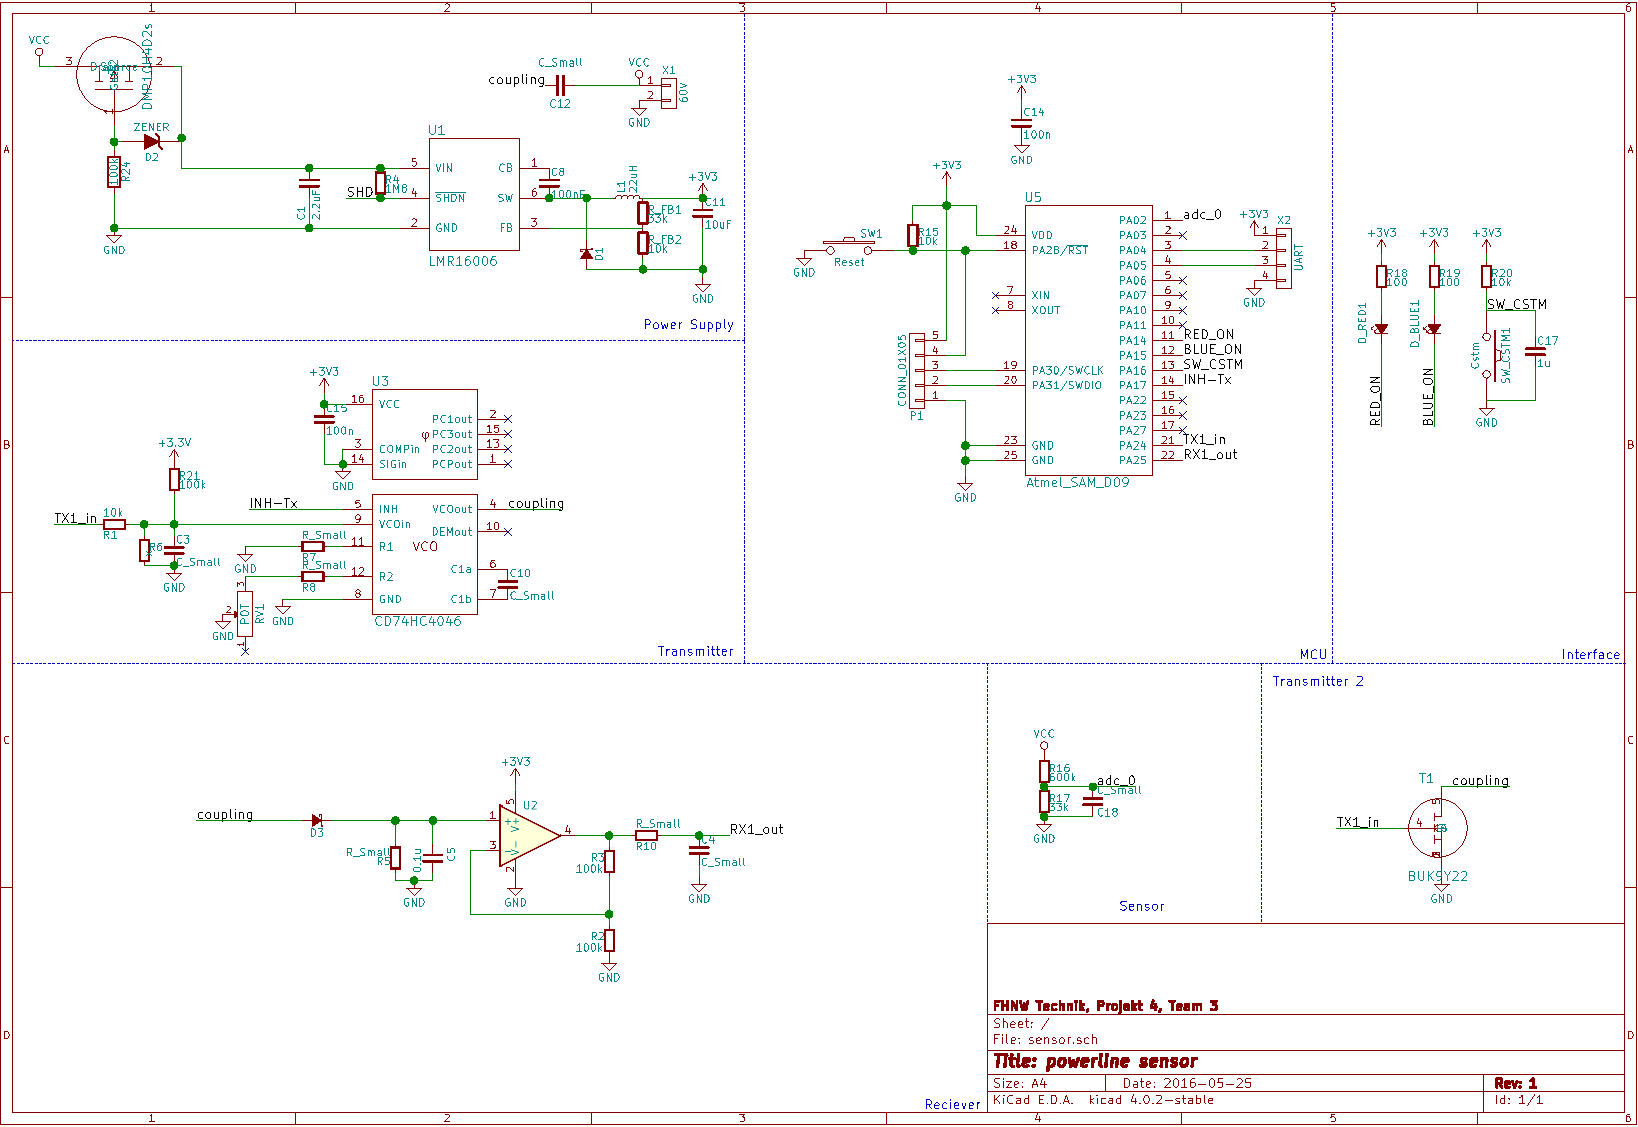
\includepdf[angle=90]{includes/a4.pdf}

Lastly, we can also include landscape A3 documents like so:

\begin{verbatim}
\begin{a3pages}
    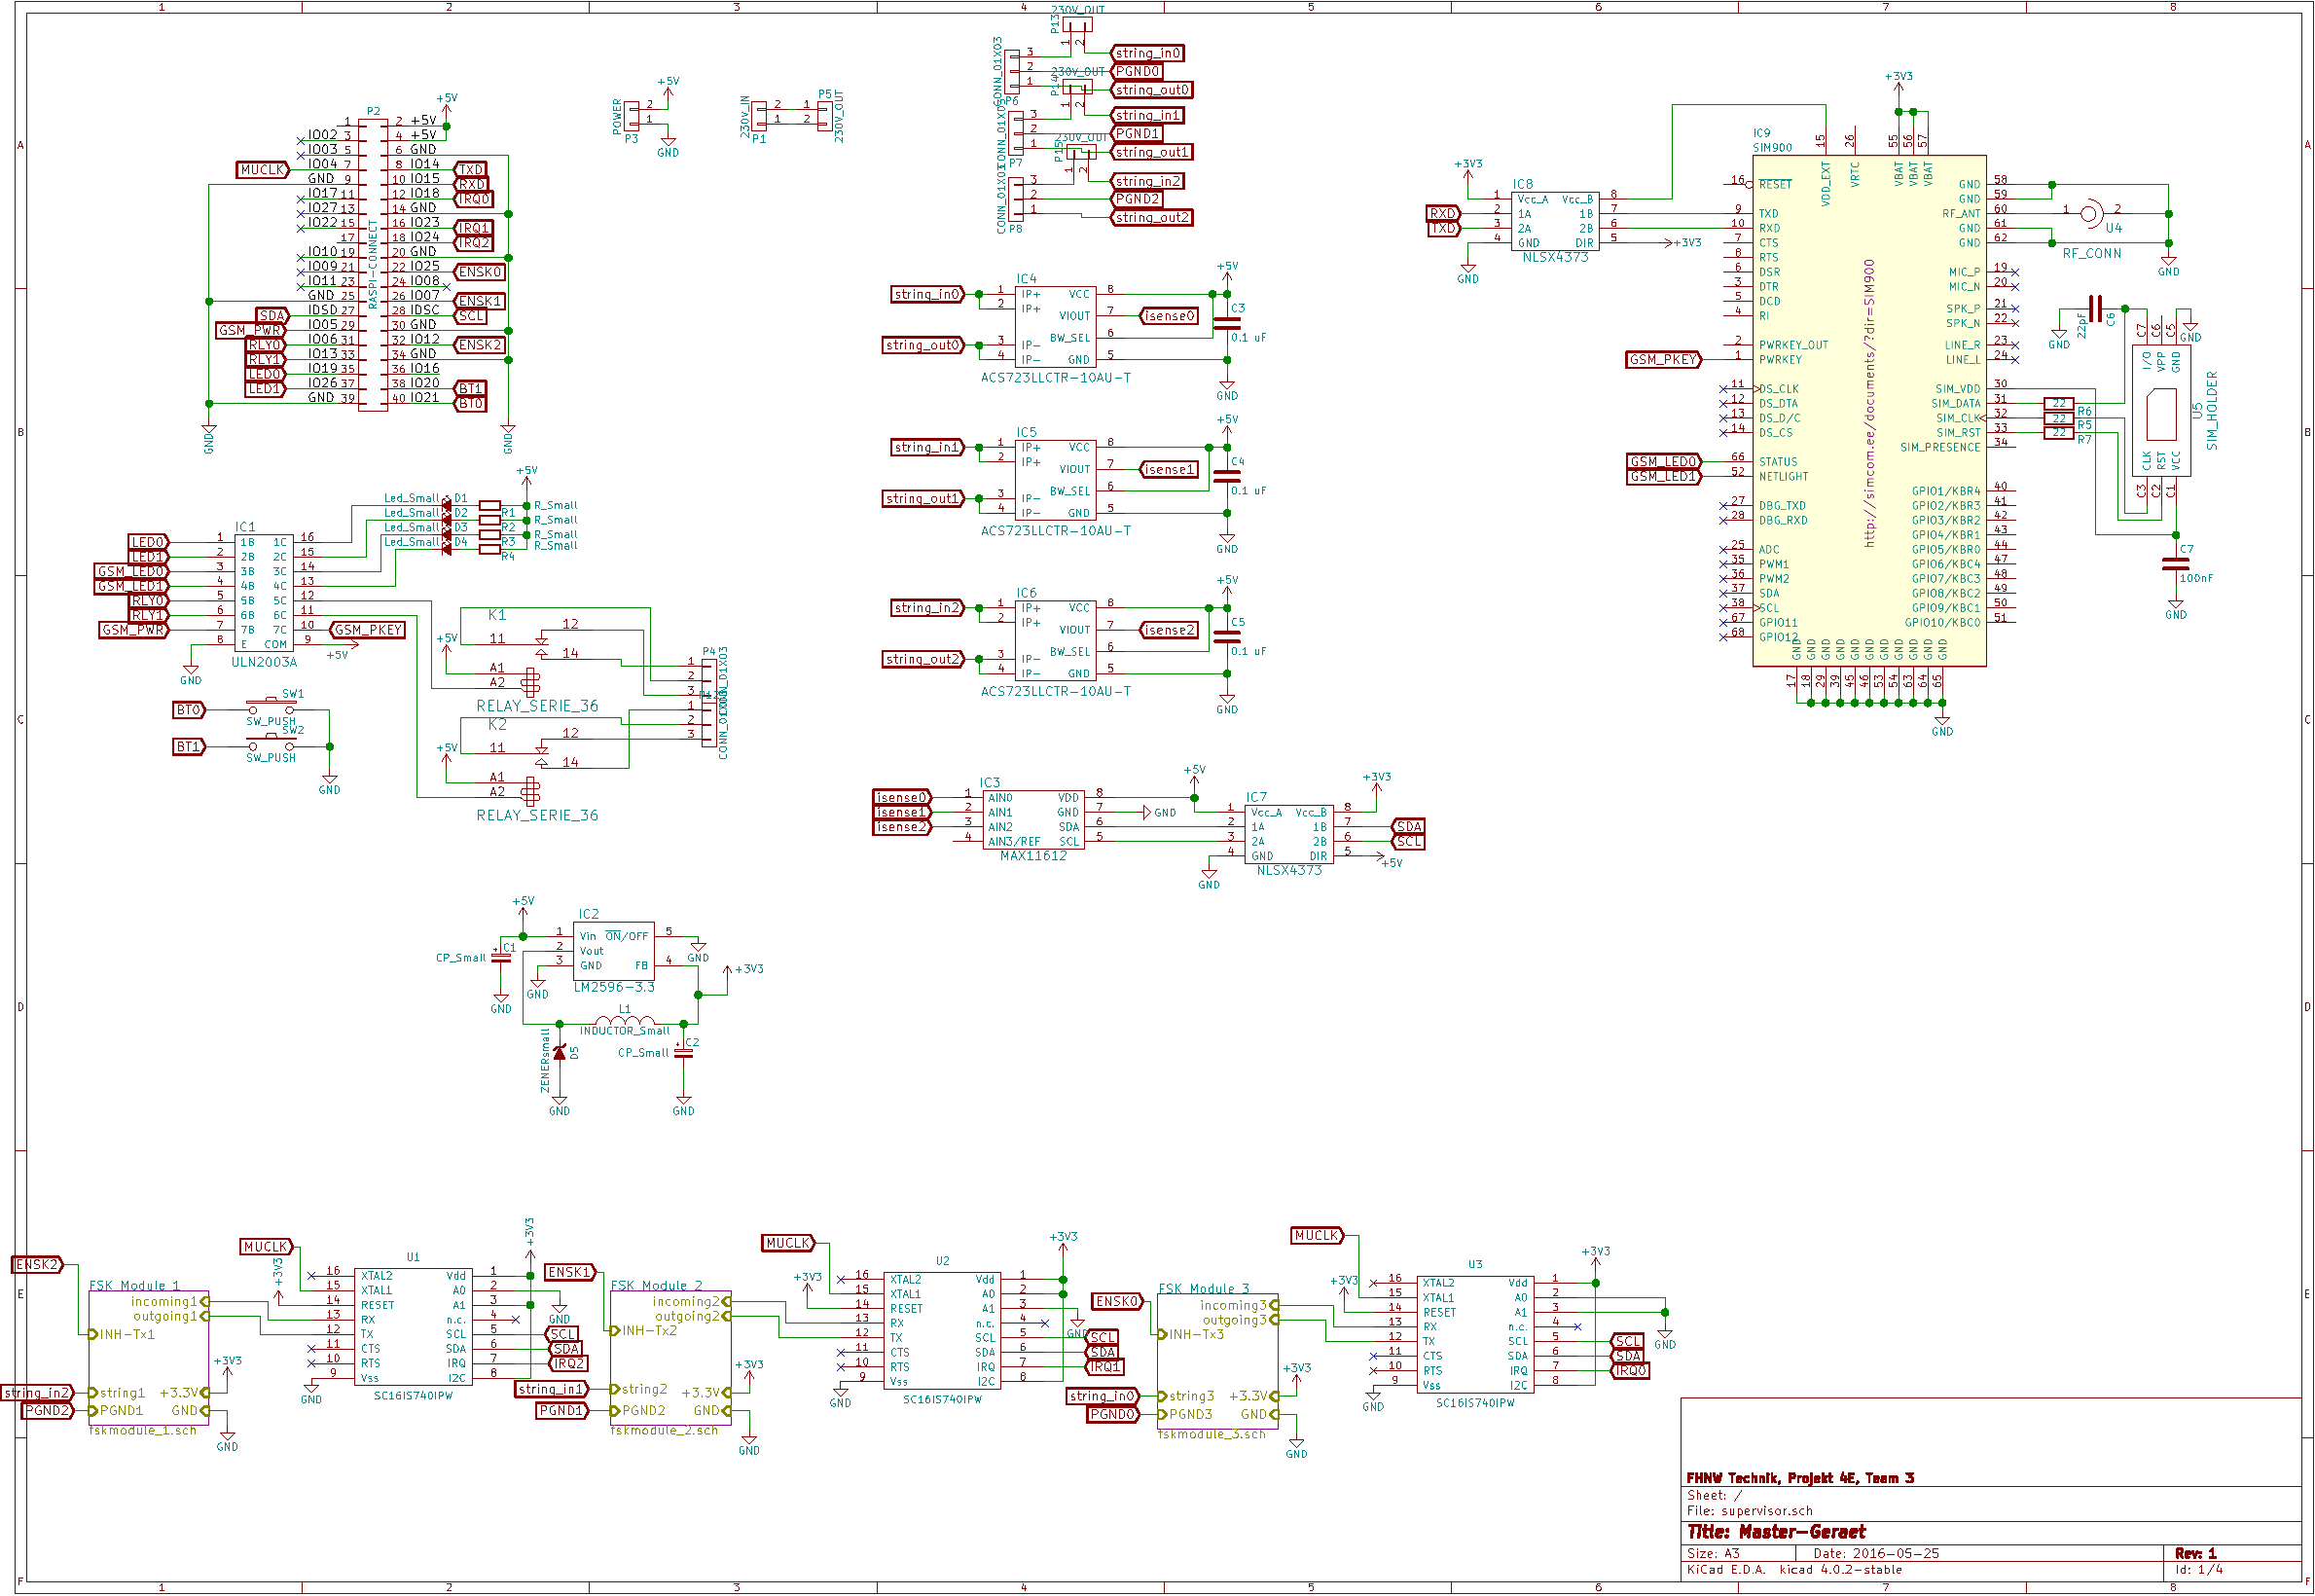
\includepdf{includes/a3.pdf}
\end{a3pages}
\end{verbatim}

This uses the \code{a3pages} package by me, available at 
\href{https://github.com/alpenwasser/TeX/tree/master/A3Pages}
     {\nolinkurl{https://github.com/alpenwasser/TeX/tree/master/A3Pages}}

\begin{a3pages}
    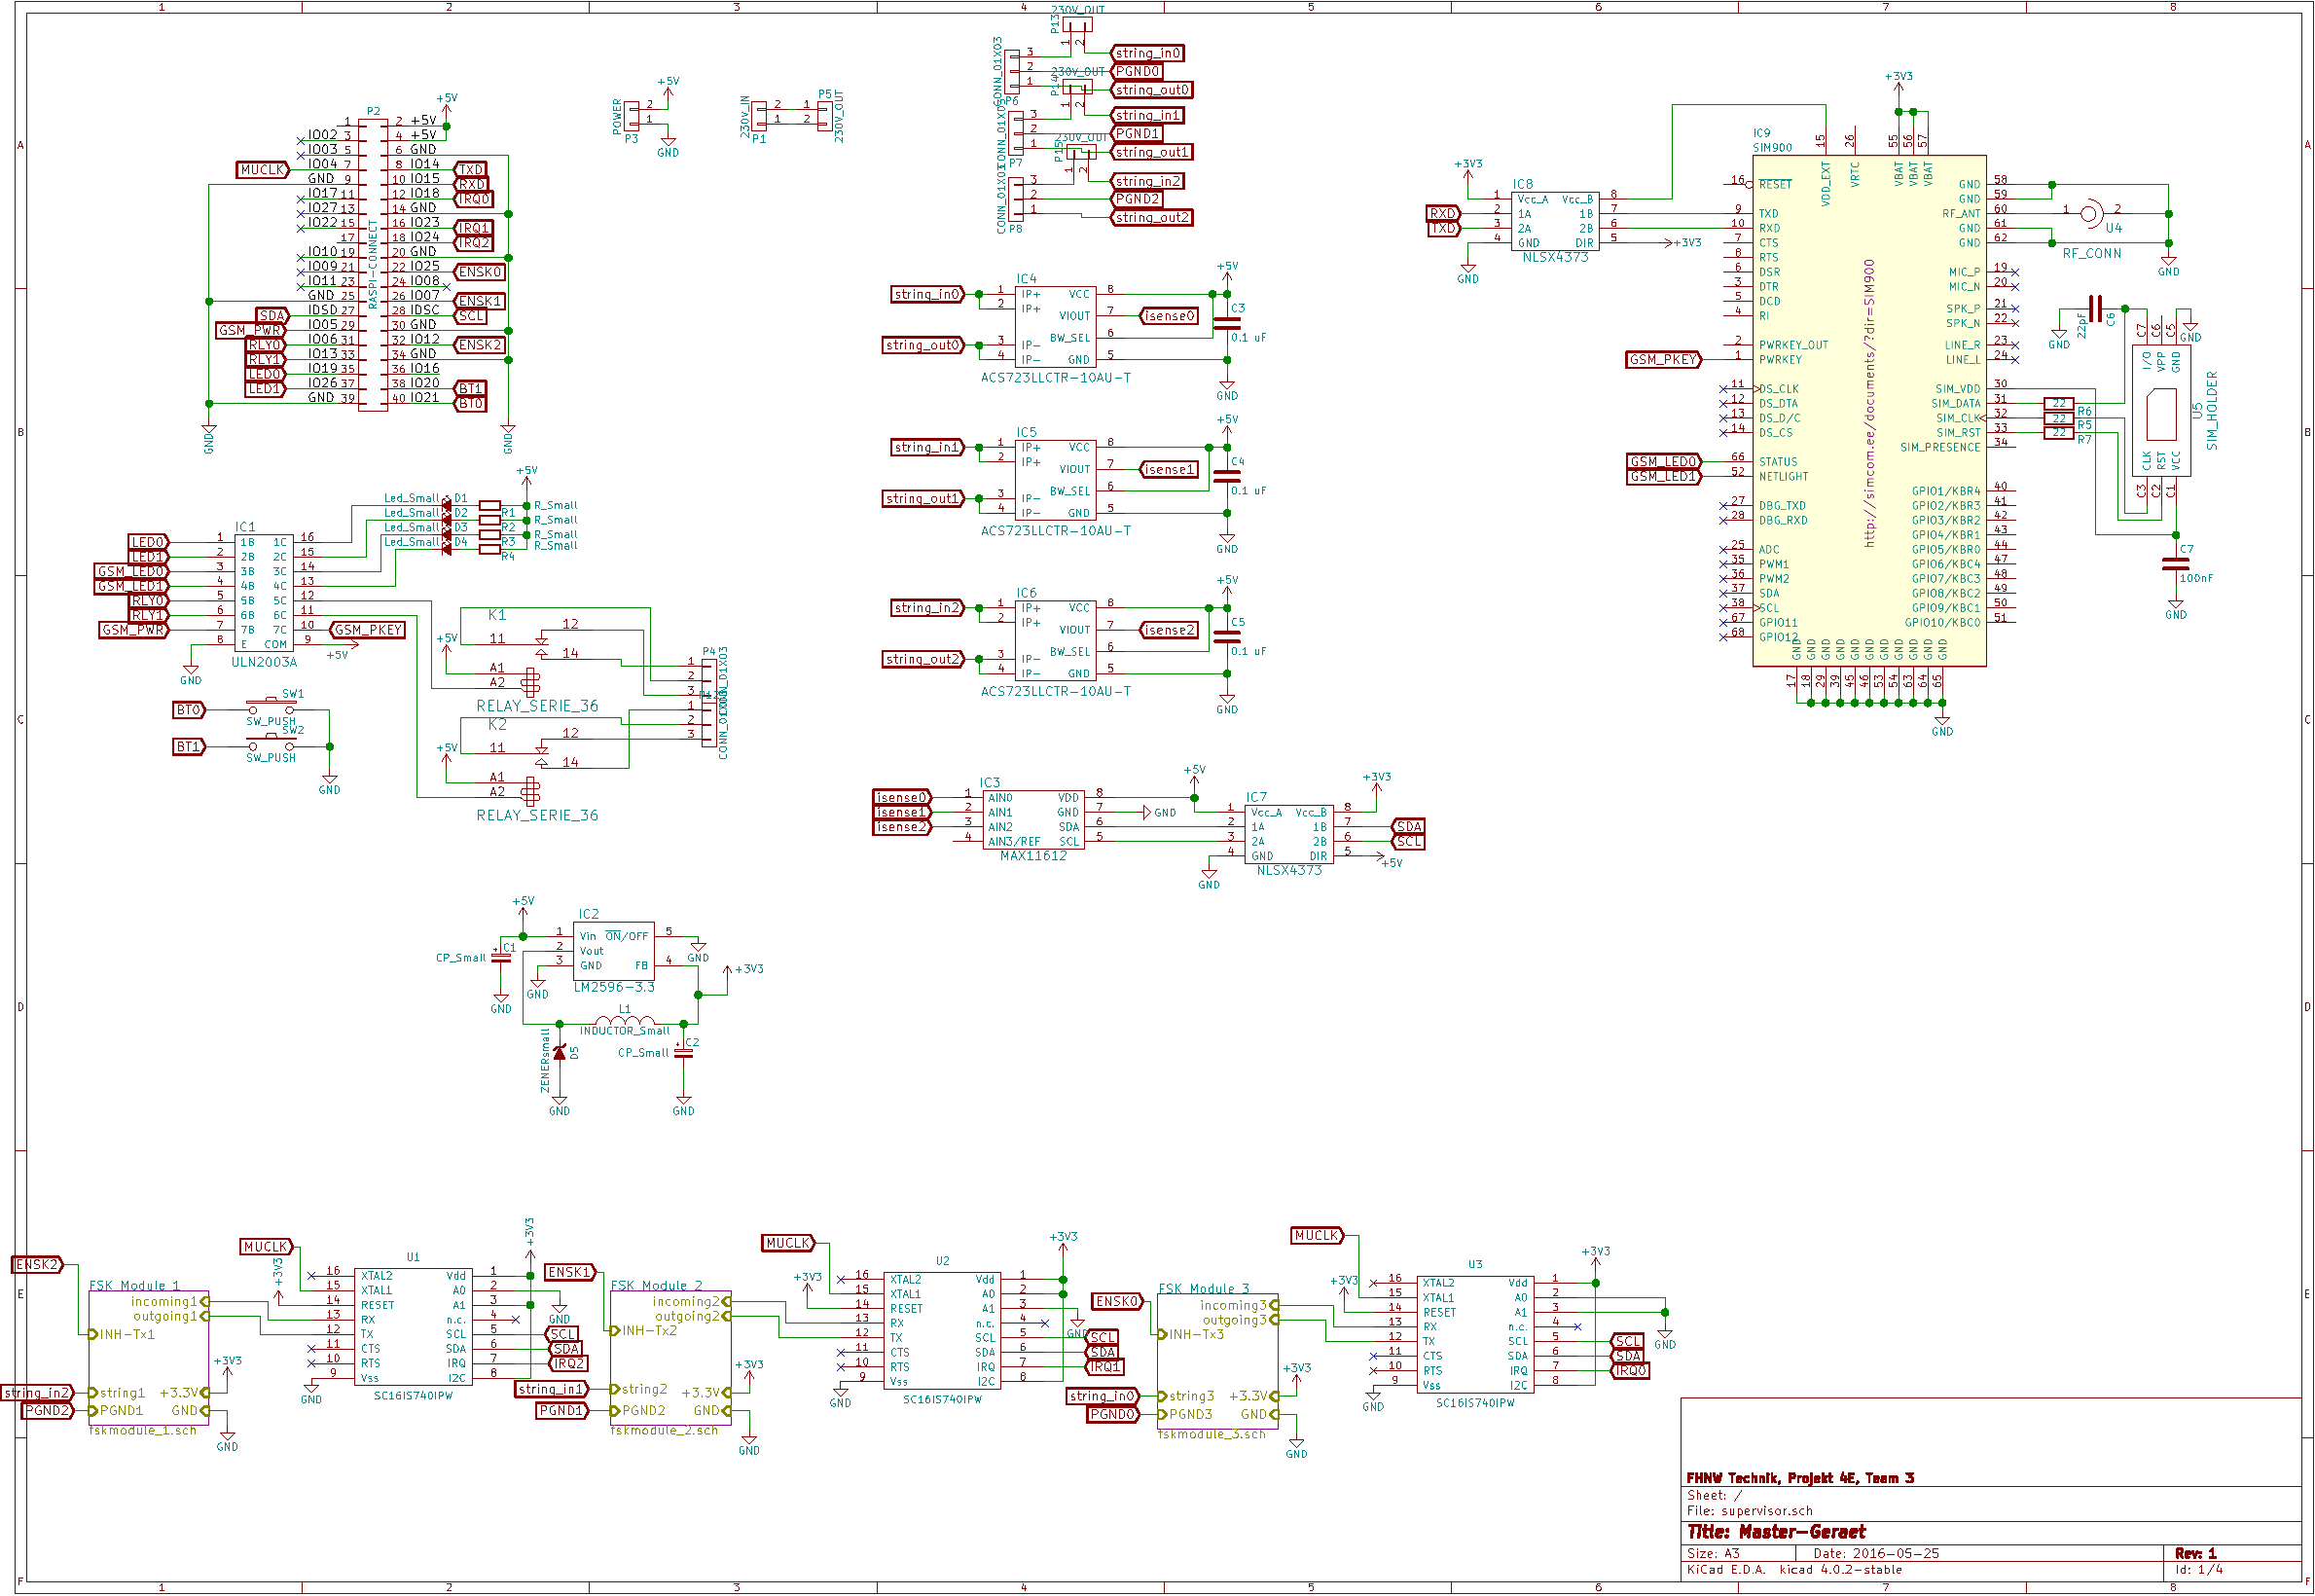
\includepdf{includes/a3.pdf}
\end{a3pages}


% -------------------------------------------------------------------------- %
\clearpage
\section{Ti\emph{k}Z}
\label{sec:tikz}
% -------------------------------------------------------------------------- %

Lastly, we're  going to include PDF  documents by using Ti\emph{k}Z. We  put a
\code{clearpage} command  before and after the  \code{tikzpicture} environment
so that the PDF is put on a separate page.

Notice that the  page number of the  main document is still  visible below the
included \code{tikzpicture}. The same would go  for any headers and other page
decoration. This may be desirable or not; up to you.

\emph{Note:} The use of \code{pdfpagewidth}  might cause problems with certain
\TeX{}  engines. In those  cases, simply  replace it  with a  manually defined
length, like \code{297mm} or whatever is appropriate.

\begin{verbatim}
\clearpage
\begin{tikzpicture}[overlay,remember picture]
    \node at (current page.center)
    {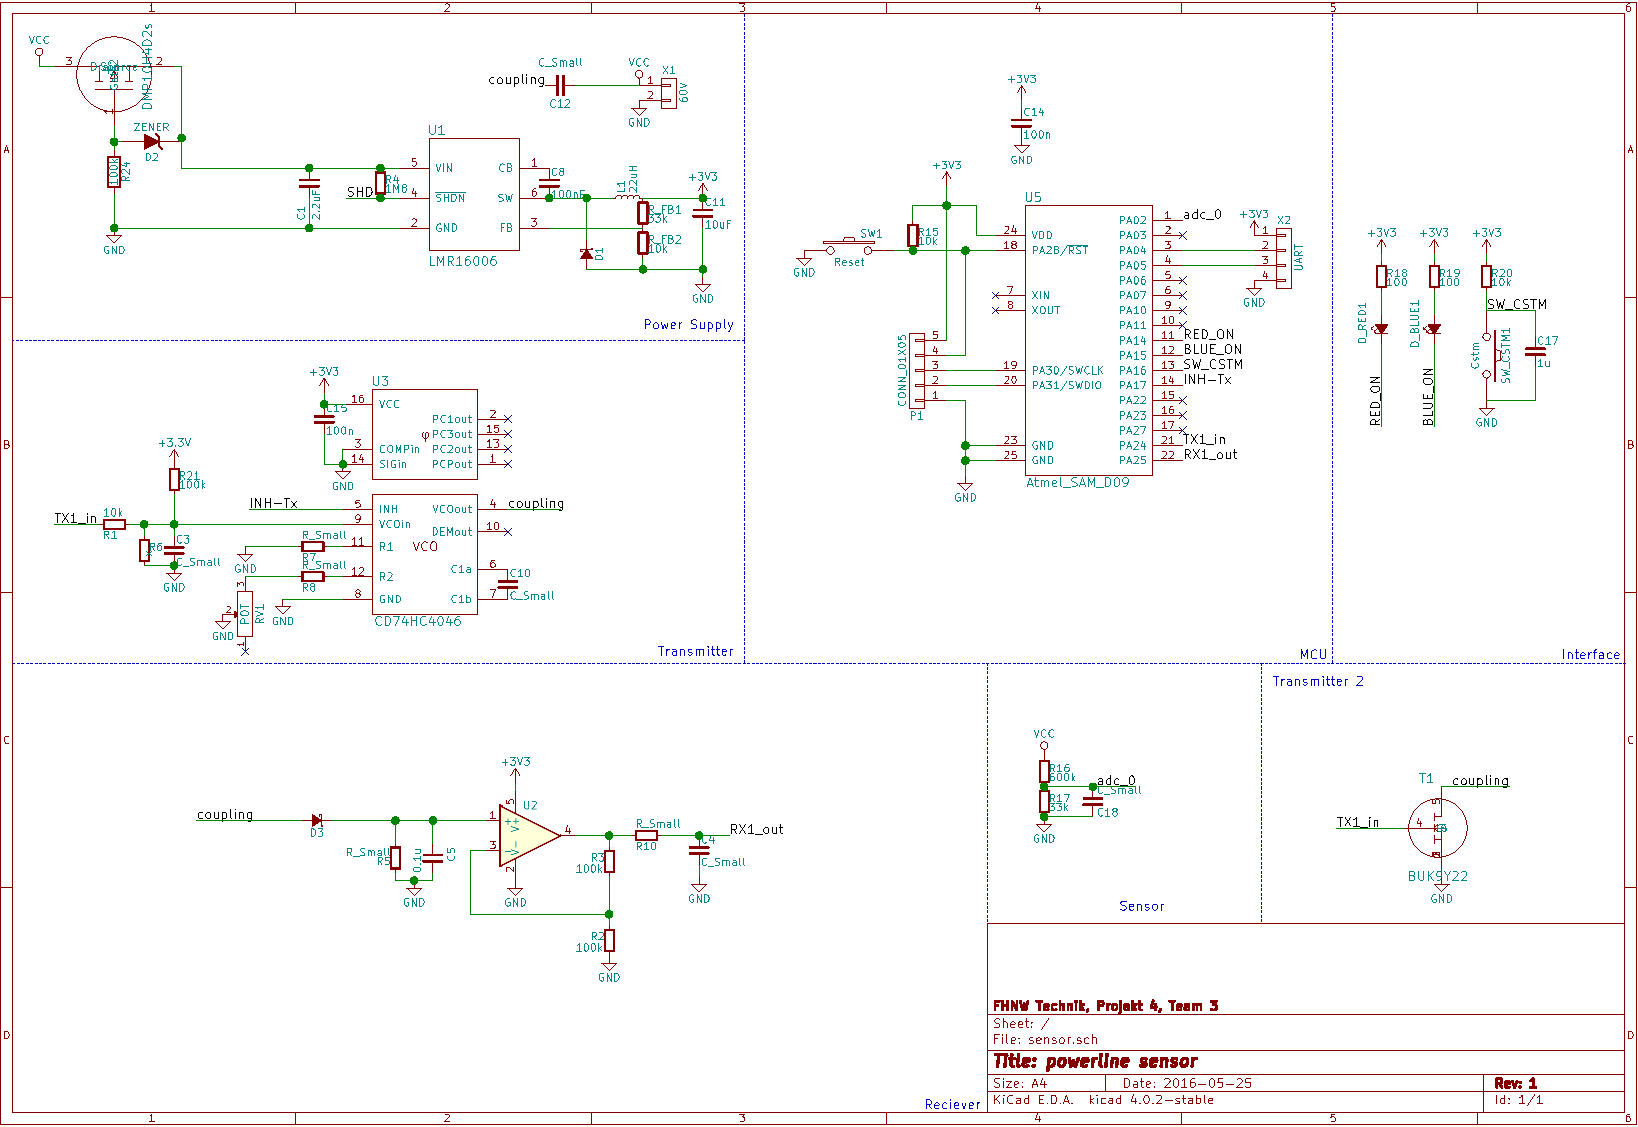
\includegraphics[angle=90,width=0.95\pdfpagewidth]{includes/a4.pdf}};
\end{tikzpicture}
\clearpage
\end{verbatim}

\clearpage
\begin{tikzpicture}[overlay,remember picture]
    \node at (current page.center)
    {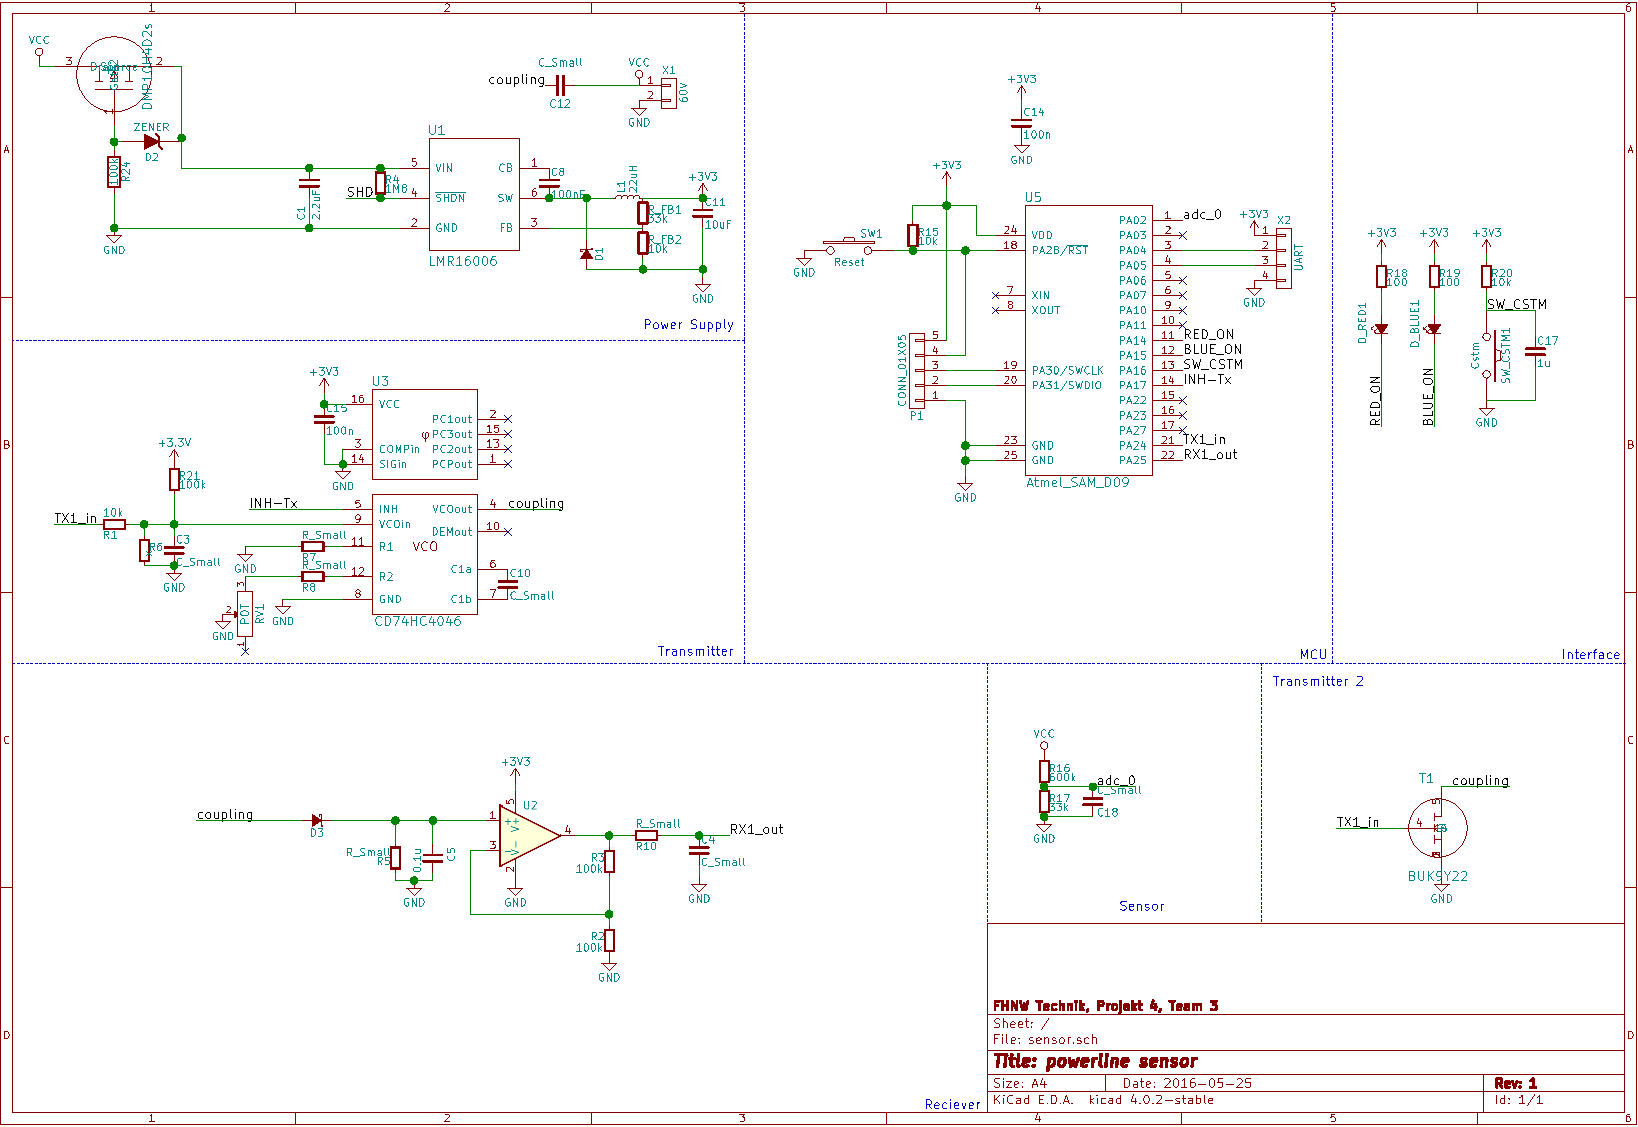
\includegraphics[angle=90,width=0.95\pdfpagewidth]{includes/a4.pdf}};
\end{tikzpicture}
\clearpage

The next page is produced with the help of the \code{pdflscape} package:

\begin{verbatim}
% In preamble:
\usepackage{pdflscape}
% In document:
\begin{landscape}
    \begin{tikzpicture}[overlay,remember picture]
        \node[xshift=178mm,yshift=-28mm] at (current page.center)
        {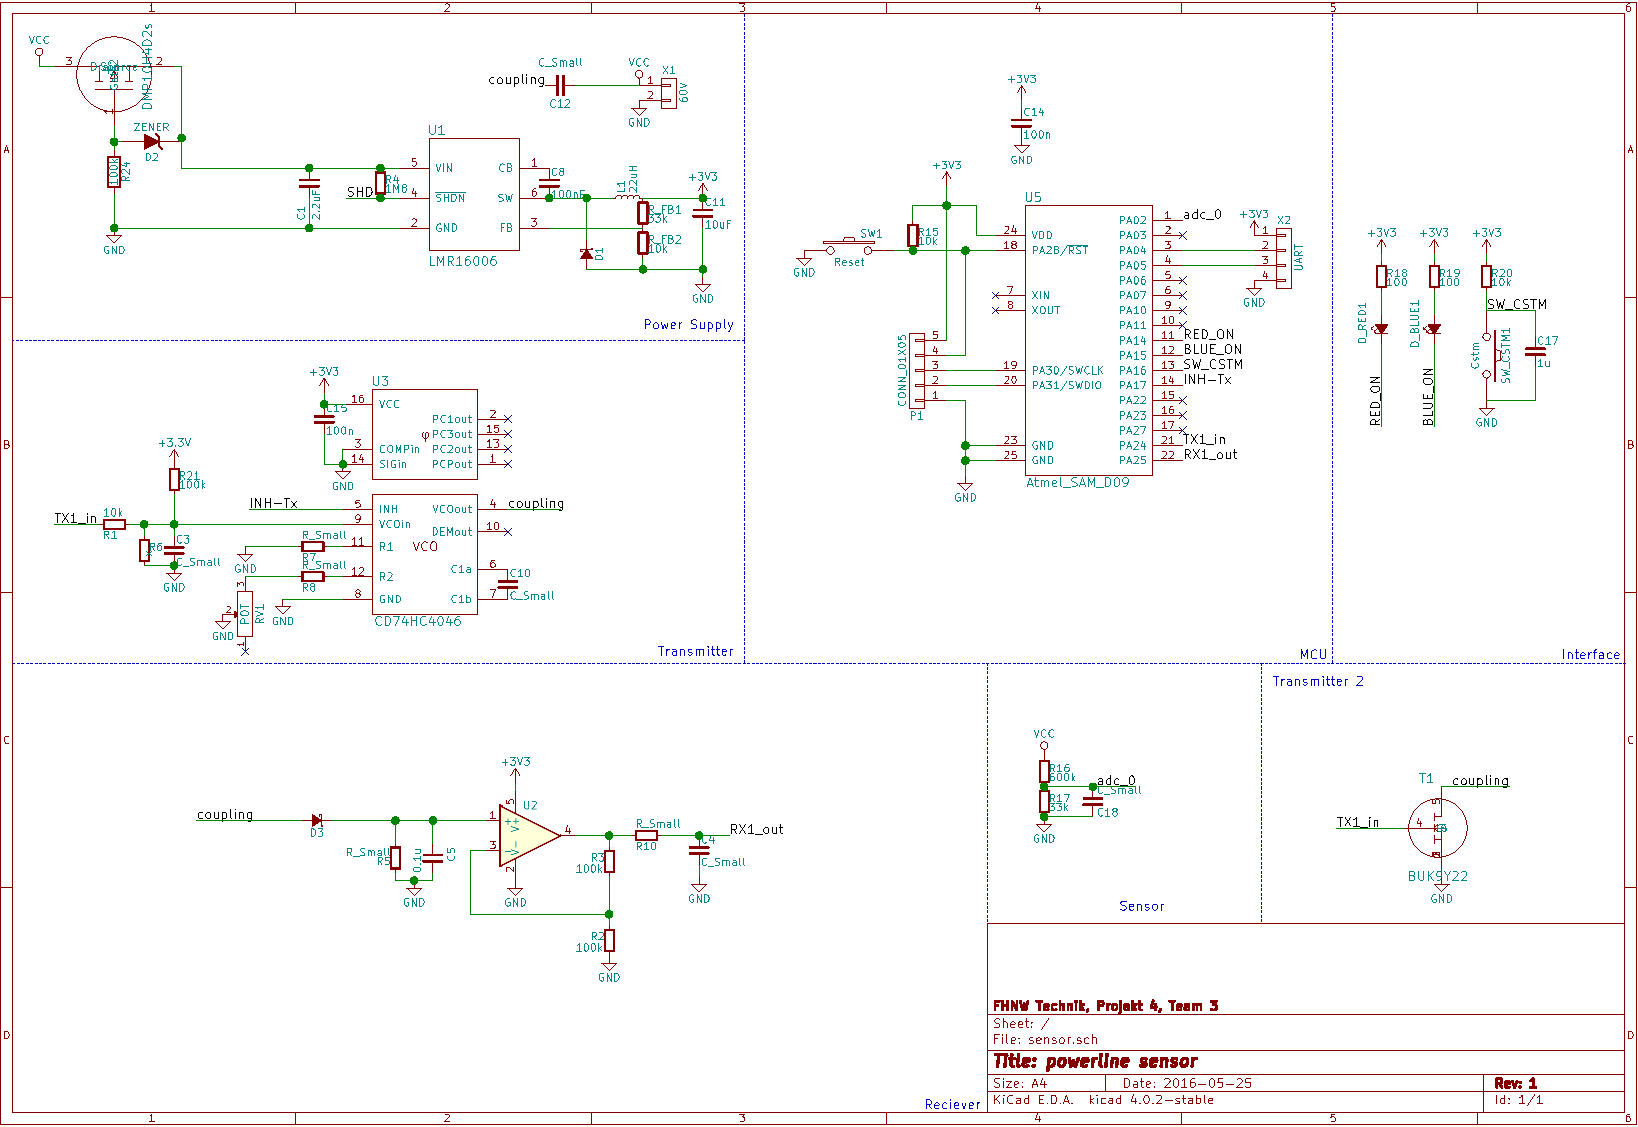
\includegraphics[width=0.95\pdfpageheight]{includes/a4.pdf}};
    \end{tikzpicture}
\end{landscape}
\end{verbatim}

Note  the \code{xshift}  and \code{yshift}  arguments to  the \code{node}. The
\code{pdflscape}  package   seems  to  interfere   with  the  page   nodes  of
Ti\emph{k}Z. I  haven't  been  able  to  find a  combination  of  anchors  and
nodes  which correctly  places the  included  pdf on  the center  of the  page
automaticlly.

\begin{landscape}
    \begin{tikzpicture}[overlay,remember picture]
        \node[xshift=178mm,yshift=-28mm] at (current page.center)
        {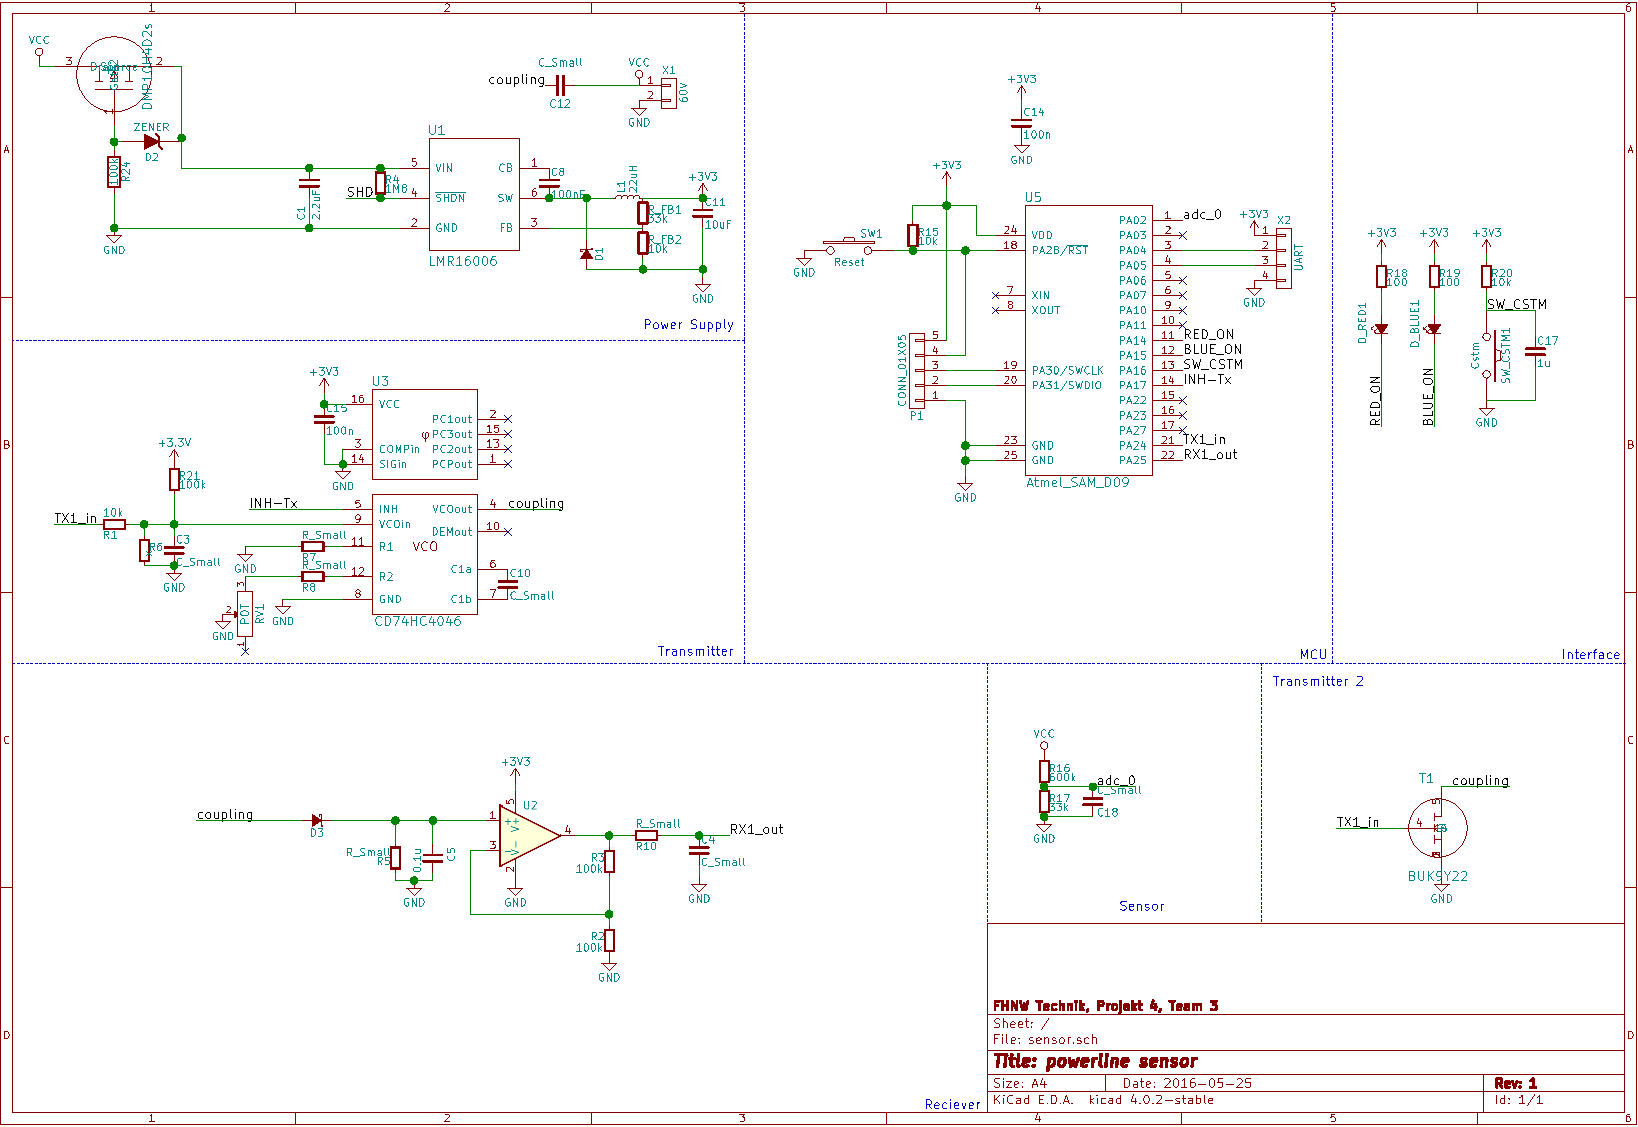
\includegraphics[width=0.95\pdfpageheight]{includes/a4.pdf}};
    \end{tikzpicture}
\end{landscape}

Lastly,  we shall  include an  A3 landscape  document as  above, but  with the
Ti\emph{k}Z technique:

\begin{verbatim}
\begin{a3pages}
    \begin{tikzpicture}[overlay,remember picture]
        \node at (current page.center)
        {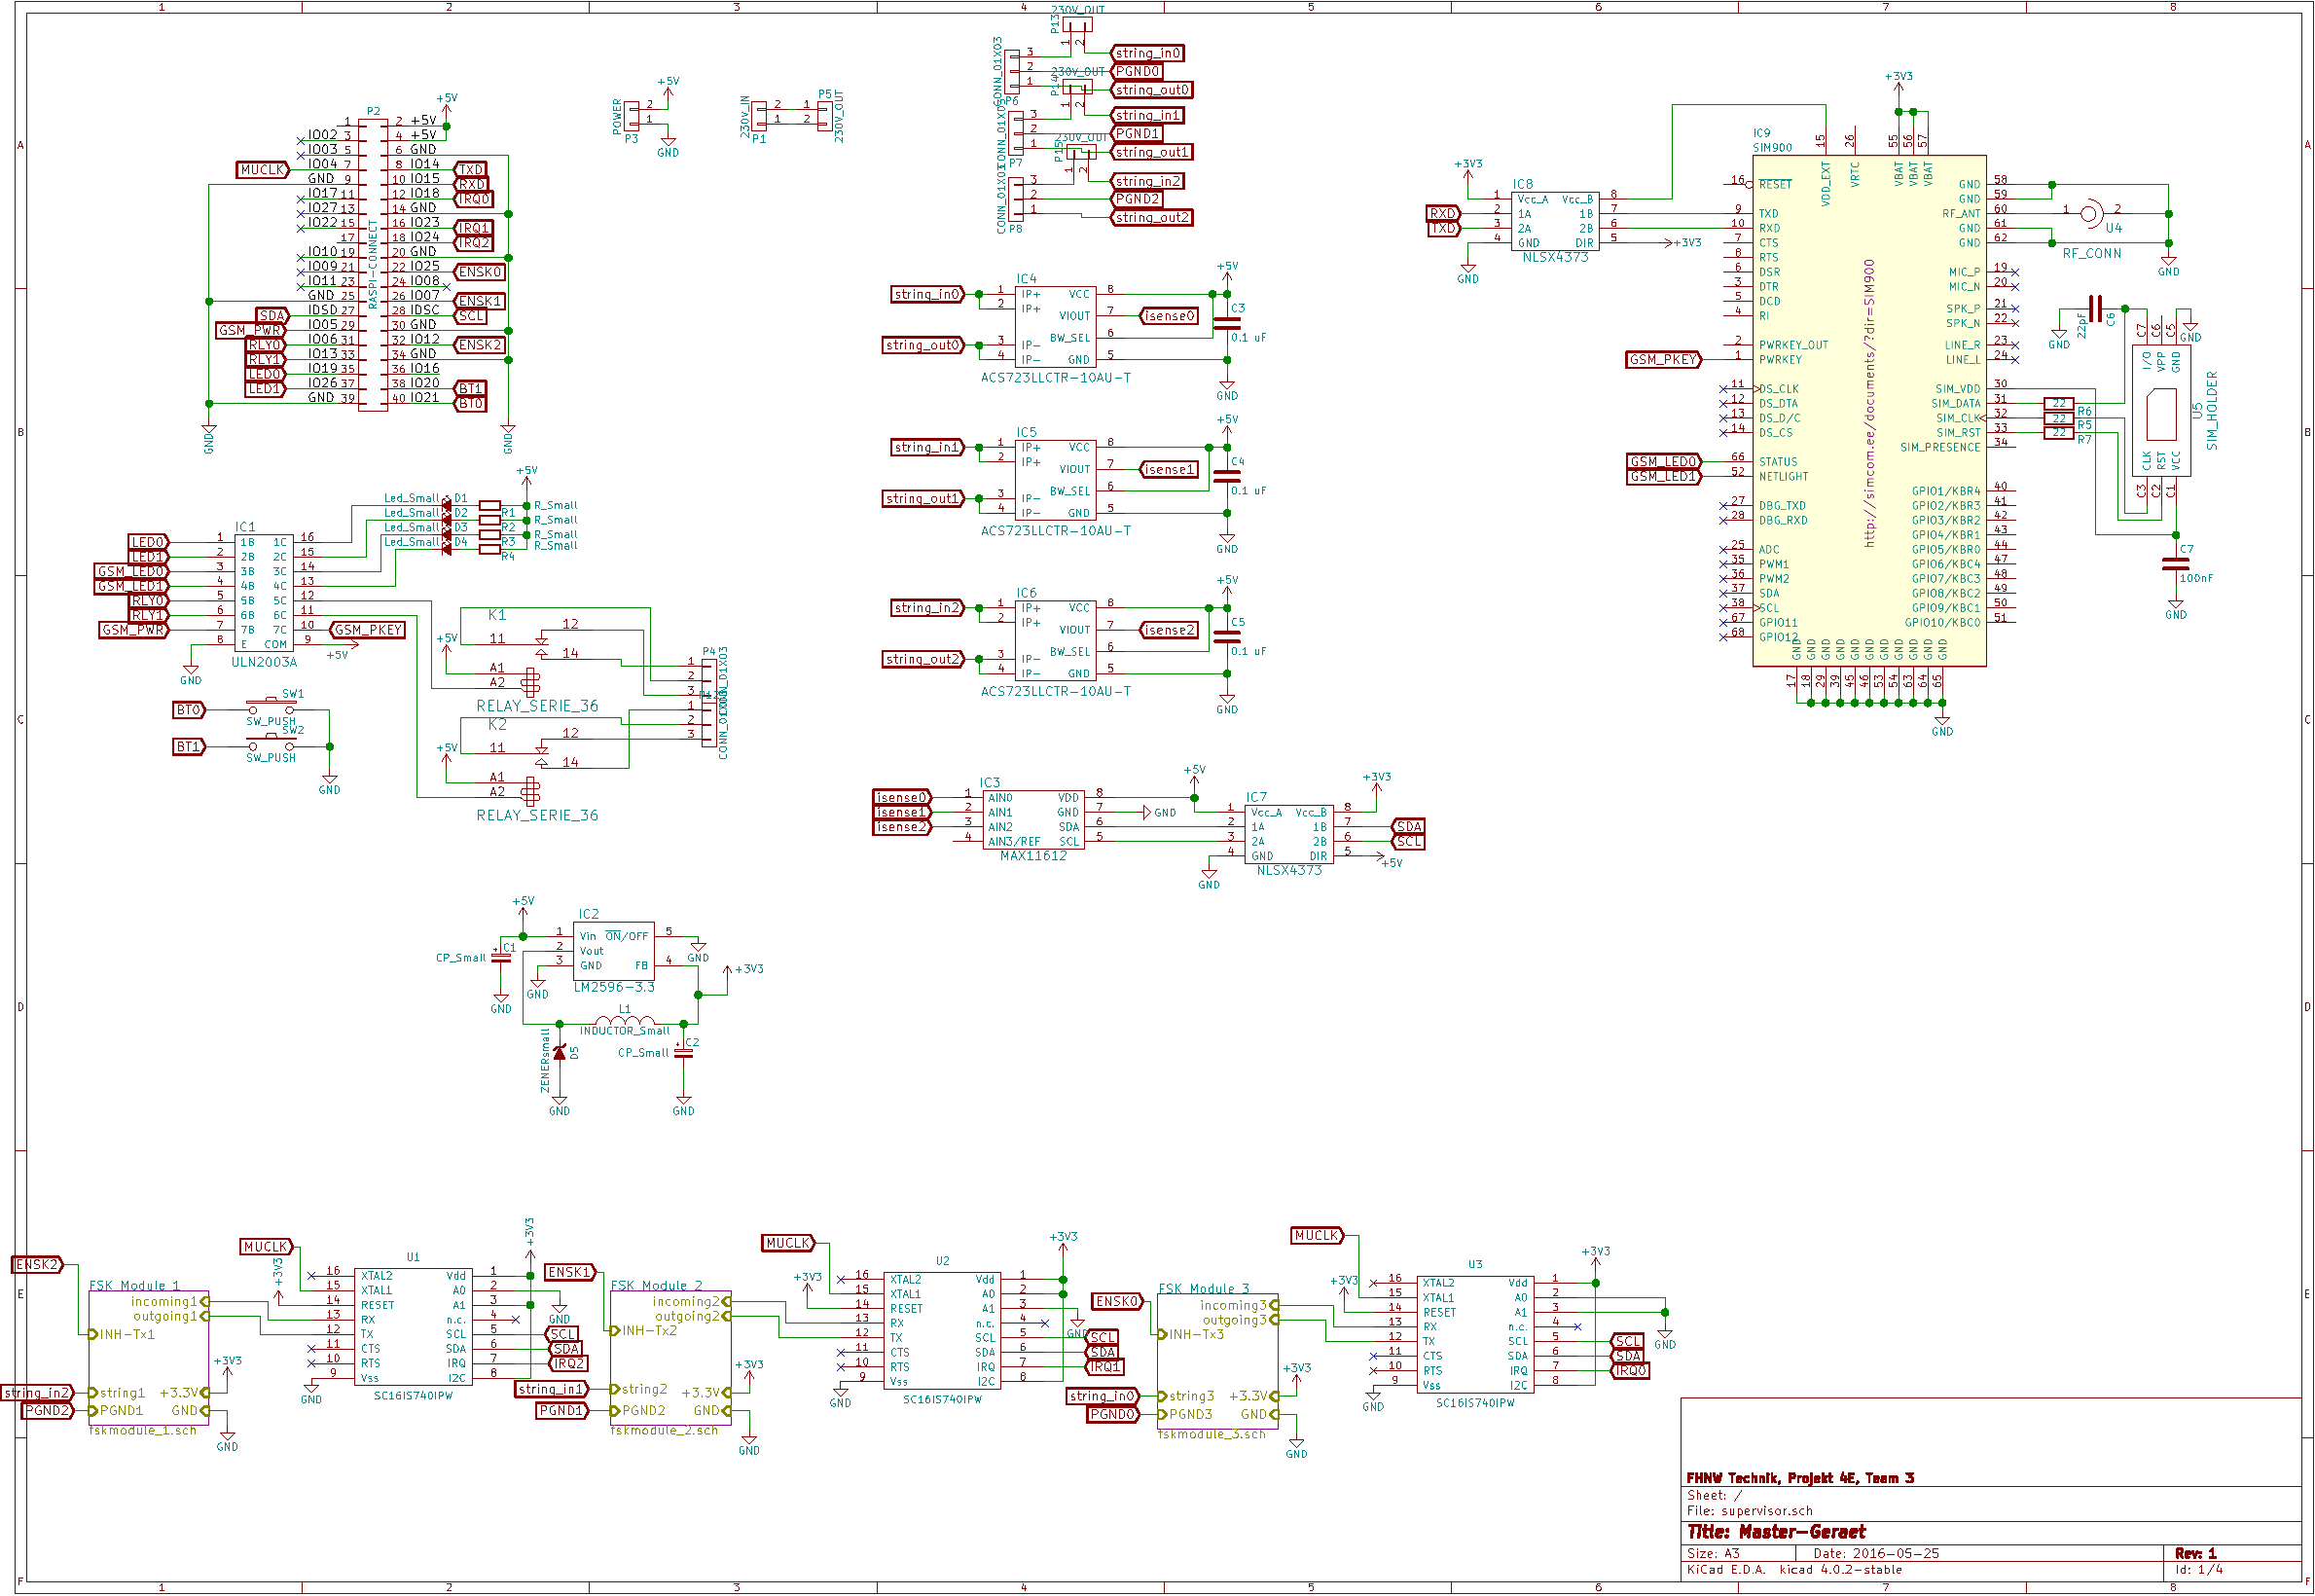
\includegraphics[width=\pdfpagewidth]{includes/a3.pdf}};
    \end{tikzpicture}
\end{a3pages}
\end{verbatim}

Again, note that the page number (\emph{19}) is still present.

\begin{a3pages}
    \begin{tikzpicture}[overlay,remember picture]
        \node at (current page.center)
        {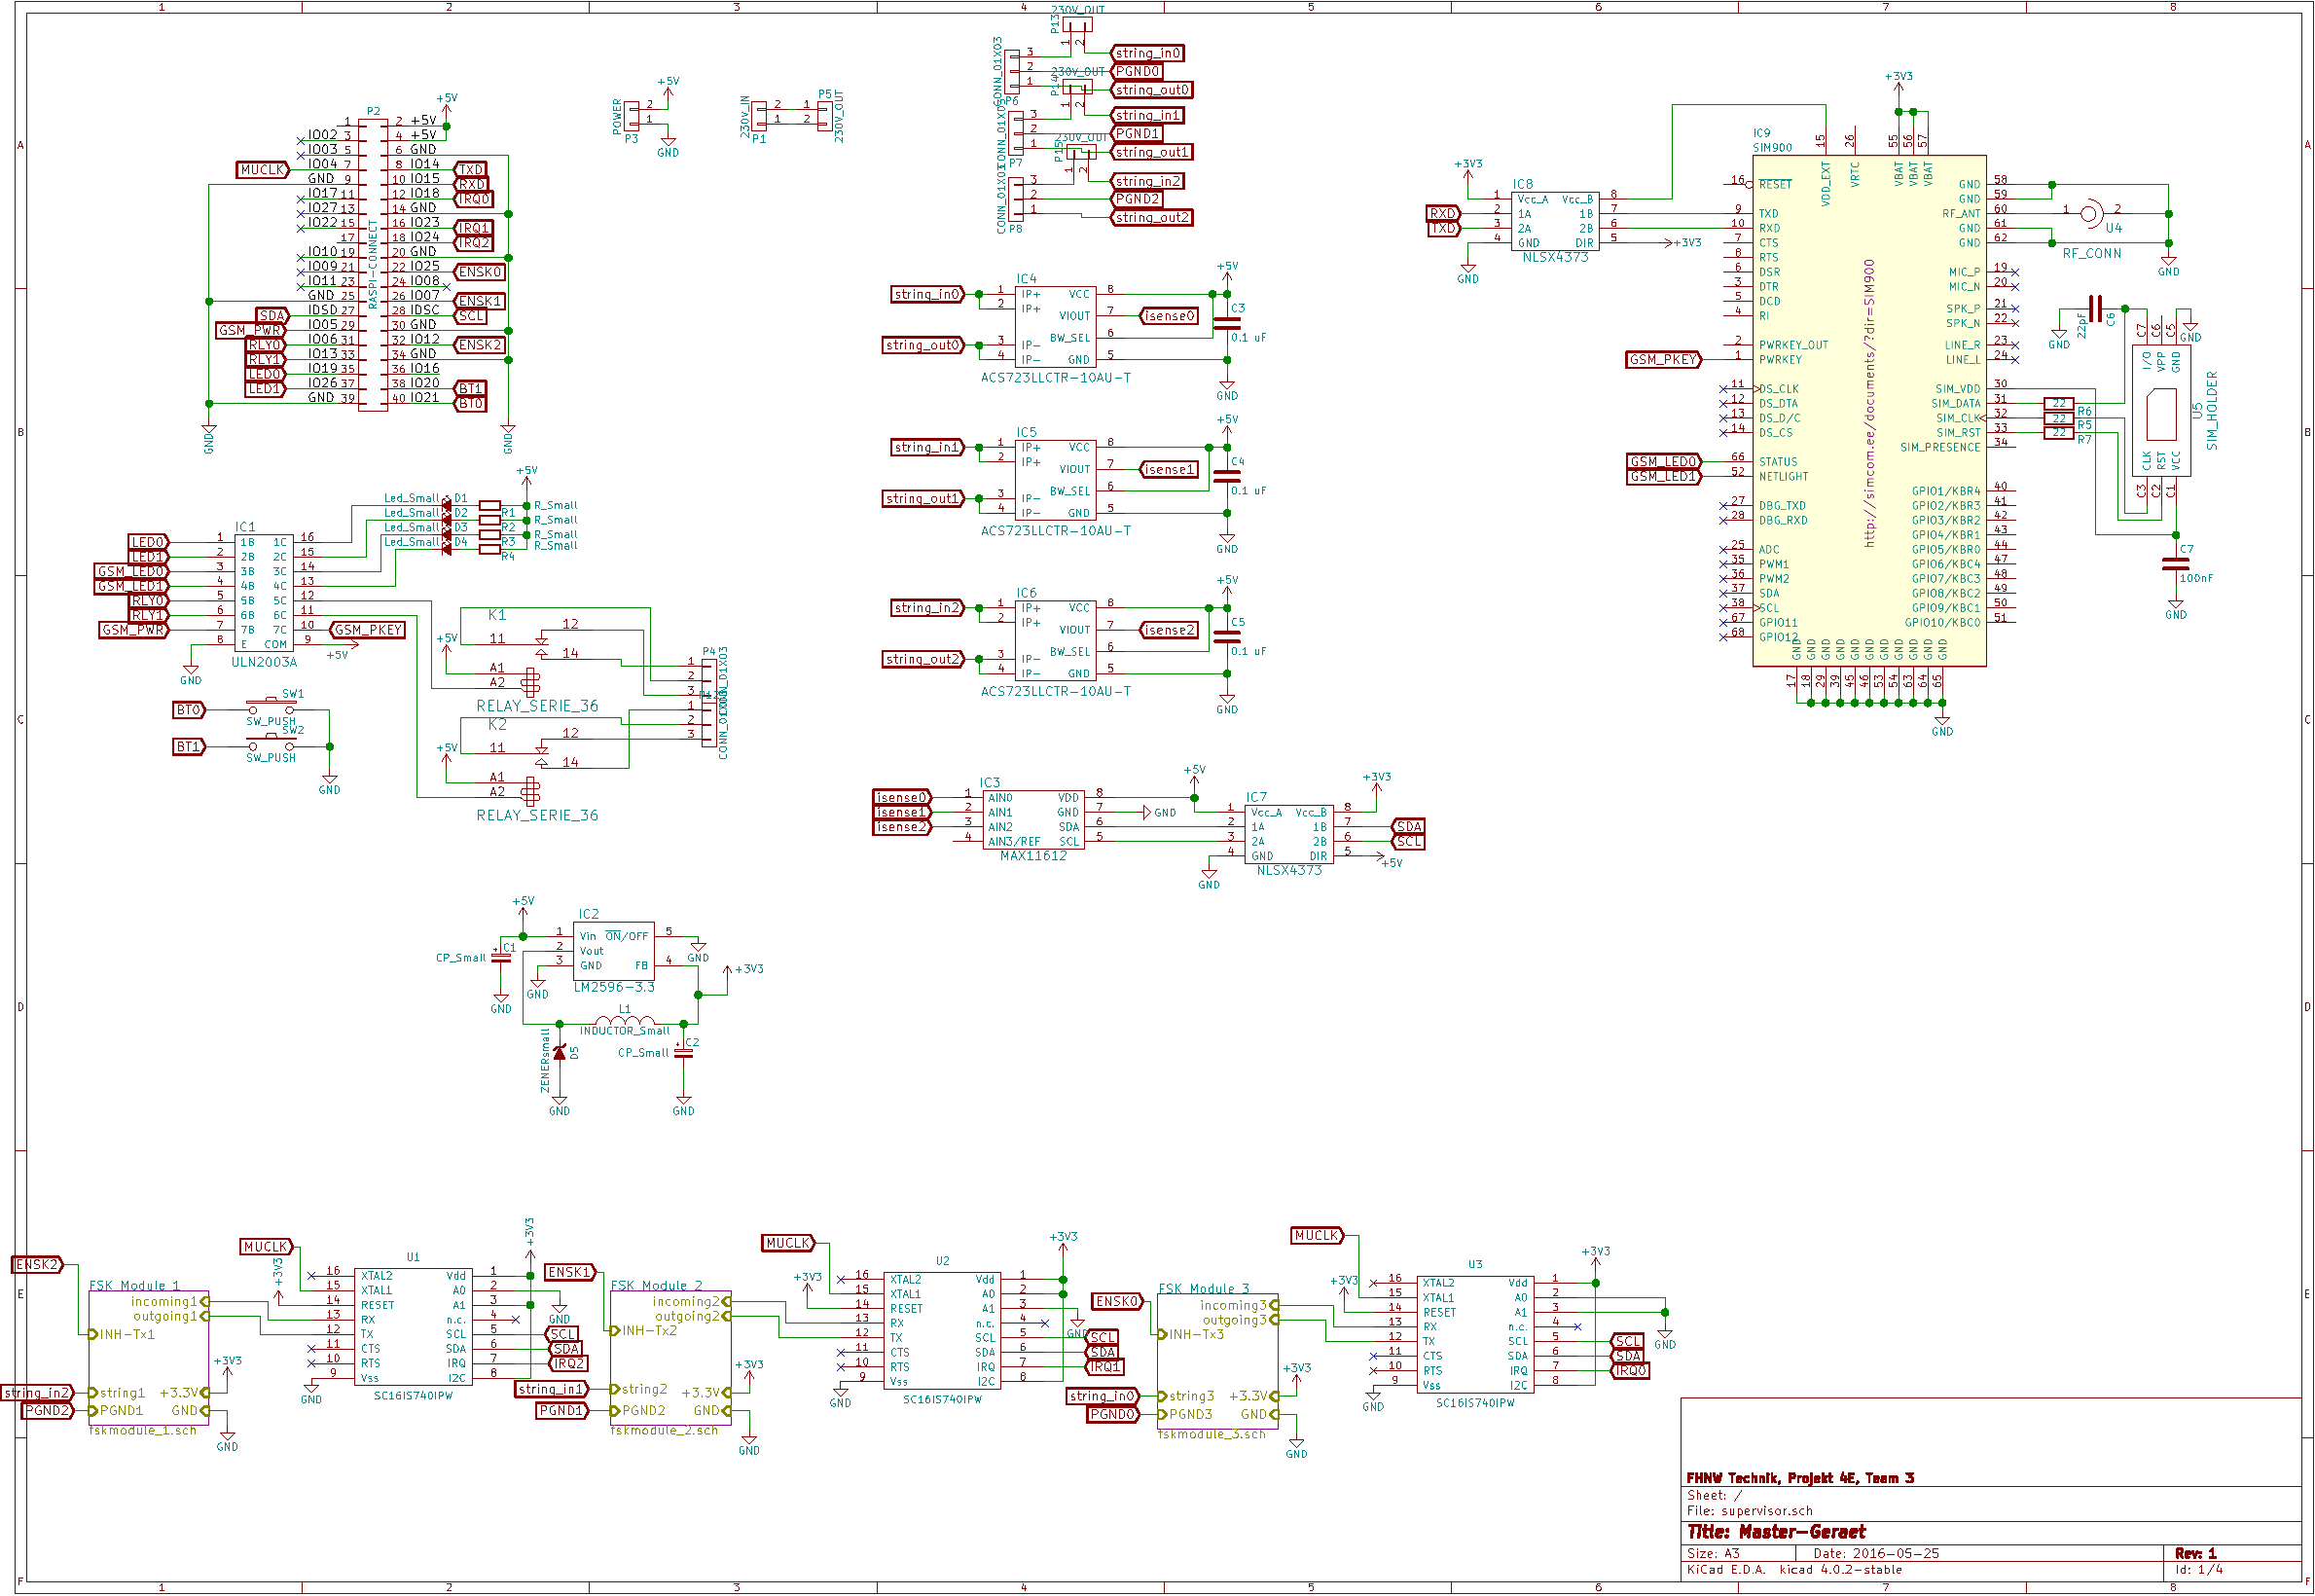
\includegraphics[width=\pdfpagewidth]{includes/a3.pdf}};
    \end{tikzpicture}
\end{a3pages}
\end{document}
